%---------------------------------------------------------------------%
%  LaTeX Course Notes Template                                        %
%                                                                     %
%  Copyright (C) 2012 Zev Chonoles                                    %
%  zevchonoles@gmail.com                                              %
%  http://math.uchicago.edu/~chonoles/                                %
%                                                                     %
%  Please leave this information in the source code as                %
%  attribution if you choose to edit or redistribute this file.       %
%                                                                     %
%  This work is licensed under the Creative Commons Attribution-      %
%  ShareAlike 3.0 Unported License. To view a copy of this license,   %
%  visit http://creativecommons.org/licenses/by-sa/3.0/.              %
%                                                                     %
%---------------------------------------------------------------------%

\documentclass[11pt]{article}






%----------%
%  Basics  %
%----------%


%  Specfies basic information.
%  In the metadata section of the preamble, you can specify the subject and a list of keywords for the PDF.
%
\newcommand{\coursetitle}{Math 500 - Topology and Geometry}
\newcommand{\lecturer}{Brian Weber}
\newcommand{\notetaker}{Zach Schutzman}
\newcommand{\notetakersemail}{ianzach+notes@seas.upenn.edu}
\newcommand{\courseterm}{Fall 2017}
\newcommand{\institution}{University of Pennsylvania}


%  array provides more column styles for the tabular and array environments.
%  (http://ctan.org/pkg/array)
%
%  parskip sets block paragraphs as the default, instead of indentation.
%  (http://www.ctan.org/pkg/parskip)
%
\usepackage[margin=1in]{geometry}
\usepackage{amsmath,amssymb,amsthm,amsfonts,array,parskip}


%  Allows equation, align, gather, etc. environments to split across pages.
\allowdisplaybreaks


%  Sets date formatting to the ISO 8601 standard, YYYY-MM-DD.
\usepackage{datetime} \renewcommand{\dateseparator}{-} \yyyymmdddate






%---------%
%  Fonts  %
%---------%


%  Defines \cal for standard calligraphy, \eucal for Euler calligraphy, and \frak for Fraktur.
\usepackage{eucal}  \let\eucal\mathcal  \let\cal\CMcal  \renewcommand{\frak}{\mathfrak}


%  Removes ligatures (e.g. the connection ordinarily made between the two f's in "differentiable").
\usepackage{microtype} \DisableLigatures{encoding=*,family=*}


%  Removes extra space after periods.




%-------------------------------%
%  Environments and Sectioning  %
%-------------------------------%


%  Defines some standard theorem environments, in both numbered and non-numbered versions. The numbering of each enviroment will be reset for each lecture.
\newcounter{lecture}       \setcounter{lecture}{0}
\newcounter{tN}[lecture]   \newcounter{dN}[lecture]
\newcounter{lN}[lecture]   \newcounter{rN}[lecture]
\newcounter{cN}[lecture]   \newcounter{eN}[lecture]
\newcounter{pN}[lecture]
\newcounter{clN}[lecture]

\newtheorem*{theorem}{Theorem}          \newtheorem{theorem-N}[tN]{Theorem}
\newtheorem*{lemma}{Lemma}              \newtheorem{lemma-N}[lN]{Lemma}
\newtheorem*{corollary}{Corollary}      \newtheorem{corollary-N}[cN]{Corollary}
\newtheorem*{proposition}{Proposition}  \newtheorem{proposition-N}[pN]{Proposition}

\theoremstyle{definition}
\newtheorem*{definition}{Definition}    \newtheorem{definition-N}[dN]{Definition}
\newtheorem*{remark}{Remark}            \newtheorem{remark-N}[rN]{Remark}
\newtheorem*{example}{Example}          \newtheorem{example-N}[eN]{Example}


\newtheorem*{claim}{Claim}    \newtheorem{claim-N}[clN]{Claim}


%  Modifies the spacing above theorem environments, which is messed up when using the parskip package.
%  (http://tex.stackexchange.com/questions/22119)
%
\makeatletter \def\thm@space@setup{\thm@preskip=\parskip \thm@postskip=0pt} \makeatother


%  Modifies the spacing above the proof environment.
%  (http://tex.stackexchange.com/questions/49801)
%
\makeatletter \renewenvironment{proof}[1][\proofname]{\pushQED{\qed}\normalfont
	\partopsep=\z@skip \topsep=\z@skip \trivlist \item[\hskip\labelsep\itshape #1\@addpunct{.}]
	\ignorespaces}{\popQED\endtrivlist\@endpefalse} \makeatother


%  Removes extra space before and after section headings.
\usepackage[compact]{titlesec}






%-------------------------%
%  Pictures and Diagrams  %
%-------------------------%


%  Allows for the use of colors.
%  (http://www.ctan.org/pkg/xcolor)
%
\usepackage[usenames,dvipsnames]{xcolor}
\definecolor{myred}{rgb}{0.9,0.2,0.2}
\definecolor{mygreen}{rgb}{0.2,0.6,0.2}
\definecolor{myblue}{rgb}{0.2,0.2,0.8}


%  graphicx provides advanced graphics options.
%  (http://ctan.org/pkg/graphicx)
%
\usepackage{graphicx}


%  tikz is for drawing all sorts of pictures and diagrams.
%  tikz-cd makes creating commutative diagrams in tikz a bit easier.
%  (http://www.ctan.org/pkg/pgf)
%  (http://www.ctan.org/pkg/tikz-cd)
%
\usepackage{tikz}
\usepackage{tikz-cd}
\usepackage{pgf,pgfplots}
\usetikzlibrary{arrows,calc,decorations,decorations.markings,fadings,positioning,patterns,shapes}
\tikzset{>=latex}
\tikzstyle{mypoint}=[inner sep=0pt,outer sep=0pt,minimum size=5pt,fill,circle]


\definecolor{ttqqqq}{rgb}{0.2,0.,0.}
\definecolor{ffffff}{rgb}{1.,1.,1.}
%\usetikzlibrary{external}
%\tikzexternalize



%------------------------%
%  Commands and Symbols  %
%------------------------%


%  Creates commands by running over a comma-separated list. For example,
%
%     \forcsvlist{\define{\newcommand}{\textbf}{bold}}{A,B}
%
%  would create
%
%     \newcommand{\boldA}{\textbf{A}}    \newcommand{\boldB}{\textbf{B}}
%
%  (http://tex.stackexchange.com/a/5776/20882)
%
\usepackage{etoolbox}
\newcommand{\define}[4]{\expandafter#1\csname#3#4\endcsname{#2{#4}}}
\forcsvlist{\define{\DeclareMathOperator}{}{}}{im,coker,rad,nil,Ann,Ass,codim,Spec,mSpec,diam,ord,Supp,supp,disc,Ob,vol,rank,Sym,Alt,Ind}
\forcsvlist{\define{\newcommand}{\mathrm}{}}{Hom,Mor,id,GL,SL,SO,SU,U,M,Mat,Ext,Tor,Res,Cor,Inf,End,Irr,Aut,Gal,lcm,tr,sign,triv,diag,Map,op,ev,act,alg,sep,unr,nr,ab}

%  Creates commands for some names of categories in the sans-serif font.
\forcsvlist{\define{\newcommand}{\mathsf}{}}{Set,Grp,Ab,CRing,Mod,Vect,Cat,Top,PreSh,Sh,Sch,Nat,Fun,Diff}

%  Creates commands for some blackboard bold letters.
\forcsvlist{\define{\newcommand}{\mathbb}{}}{N,Z,Q,R,C,F,G,T,A,B,D}


%  Saves the section symbol, paragraph symbol, Hungarian accent, and Scandanavian O in the macros \SS, \PP, \HH, and \OO, then redefines \S, \P, \H, and \O to be the corresponding blackboard bold letters.
%
\let\SS\S  \let\PP\P  \let\HH\H  \let\OO\O
\forcsvlist{\define{\renewcommand}{\mathbb}{}}{S,P,H,O}


%  latexsym defines some alternative versions of amssymb symbols.
%  (http://www.bakoma-tex.com/doc/latex/base/latexsym.pdf)
%
\usepackage{latexsym}


%  Defines a copyright symbol that is a bit nicer than the built-in one.
\newcommand{\mycopyrightsymbol}{\raisebox{-0.3ex}{\tikz{\node[inner sep=0pt,outer sep=0pt] at (0,0) {\textsc{c}};\draw (0,0) circle (0.18);}}}


%  Defines commands for real and complex projective space.
\newcommand{\RP}{\mathbb{R}\mathrm{P}}  \newcommand{\CP}{\mathbb{C}\mathrm{P}}


%  Defines a bordered matrix with square bracket delimiters instead of parentheses.
%  (http://tex.stackexchange.com/questions/55054)
%
\let\bbordermatrix\bordermatrix
\patchcmd{\bbordermatrix}{8.75}{4.75}{}{}
\patchcmd{\bbordermatrix}{\left(}{\left[}{}{}
\patchcmd{\bbordermatrix}{\right)}{\right]}{}{}


%  Calls one of the mathabx font families so that it is possible to use its symbols without making a global change.
%  (http://www.ctan.org/pkg/mathabx)
%  (http://tex.stackexchange.com/questions/14386)
%
\DeclareFontFamily{U}{mathb}{\hyphenchar\font45}
\DeclareFontShape{U}{mathb}{m}{n}{<5> <6> <7> <8> <9> <10> gen * mathb
	<10.95> mathb10 <12> <14.4> <17.28> <20.74> <24.88> mathb12}{}
\DeclareSymbolFont{mathb}{U}{mathb}{m}{n}


%  Defines circular arrows.
\DeclareMathSymbol{\lcirclearrow}{0}{mathb}{'366}
\DeclareMathSymbol{\rcirclearrow}{0}{mathb}{'367}
\newcommand{\leftcirclearrow}{\mathrel{\ensuremath{\raisebox{0.1ex}{\scalebox{0.9}{\rotatebox[origin=c]{90}{$\lcirclearrow$}}}}}}
\newcommand{\rightcirclearrow}{\mathrel{\ensuremath{\raisebox{0.1ex}{\scalebox{0.9}{\rotatebox[origin=c]{270}{$\rcirclearrow$}}}}}}


%  Gives semantic names for some common math symbols.
\newcommand{\iso}{\cong}
\newcommand{\htop}{\sim}
\newcommand{\htopequiv}{\simeq}
\newcommand{\cupprod}{\mathbin{\smallsmile}}
\newcommand{\capprod}{\mathbin{\smallfrown}}
\newcommand{\wedgesum}{\mathbin{\vee}}
\newcommand{\boundary}{\partial}
\renewcommand{\emptyset}{\varnothing}
\newcommand{\characteristic}{\mathrm{char}}
\newcommand{\symdiff}{\mathbin{\vartriangle}}
\newcommand{\convolute}{\mathbin{\ast}}
\newcommand{\actson}{\rightcirclearrow}
\newcommand{\actedonby}{\leftcirclearrow}
\newcommand{\directsum}{\oplus}
\newcommand{\bigdirectsum}{\bigoplus}
\newcommand{\tensor}{\otimes}
\newcommand{\bigtensor}{\bigotimes}
\newcommand{\free}{\mathbin{\ast}}
\newcommand{\bigfree}{\mathop{\ensuremath{\raisebox{-0.7ex}{\scalebox{2.3}{$\ast$}}}}}
\renewcommand{\complement}[1]{{#1}^{\mathsf{c}}}
\newcommand{\transpose}[1]{{#1}^{\textsf{T}}}
\newcommand{\union}{\cup}
\newcommand{\intersect}{\cap}
\newcommand{\transverse}{\mathrel{\raisebox{1.1ex}{$-$}\mathllap{\pitchfork\hspace{0.22mm}}}}



\def\multiset#1#2{\ensuremath{\left(\kern-.3em\left(\genfrac{}{}{0pt}{}{#1}{#2}\right)\kern-.3em\right)}}



%-----------------------------------%
%  Things Specific to Course Notes  %
%-----------------------------------%


%  Formatting for the table of contents. The first line allows for multi-column environments, the second line removes the heading "Contents".
\usepackage{multicol} \setlength{\columnsep}{3cm}
\makeatletter \renewcommand\tableofcontents{\@starttoc{toc}} \makeatother


%  Sets the page style.
\usepackage{fancyhdr}
\pagestyle{fancy}
\renewcommand{\headrulewidth}{0pt}
\renewcommand{\footrulewidth}{0.5pt}
\setlength{\headheight}{14pt}
\lfoot{\parbox[t]{1in}{\centering Last edited\\ \today}}
\cfoot{\parbox[t]{3in}{\centering \coursetitle}}
\rfoot{\parbox[t]{0.9in}{\centering Page \thepage\\ Lecture \arabic{lecture}}}


%  Sets the inputs for \maketitle.
\author{%Lectures by \lecturer\\ 
	Notes by \notetaker}
\title{\coursetitle}
\date{\institution, \courseterm}


%  Defines headings for each day's notes.
\newcommand{\classheader}[1]{\stepcounter{lecture}\newpage\section*{Lecture \arabic{lecture} (#1)}
	\phantomsection \addcontentsline{toc}{section}{Lecture \arabic{lecture} (#1)}}


%---------------------------------------%
%  Miscellaneous Additions to Template  %
%---------------------------------------%

% http://tex.stackexchange.com/questions/18359
\pgfplotsset{compat=newest}

\newcommand{\Cinfty}{\ensuremath{C^{\infty}}}
\newcommand{\Crit}{\mathrm{Crit}}
\usepackage{mathtools}
\newcommand{\Or}{\mathrm{Or}}
\renewcommand{\Re}{\mathrm{Re}}
\renewcommand{\Im}{\mathrm{Im}}
\usepackage{mathrsfs}
\newtheorem*{examples}{Examples}
\newtheorem*{exercise}{Exercise}
\usepackage{pdfpages}
\newcommand{\Lie}{\mathrm{Lie}}
\newcommand{\Diffeo}{\mathrm{Diffeo}}

\newcommand{\connection}{\nabla}
\newcommand{\new}{\mathrm{new}}


\newcommand{\review}{{\huge\color{myred}{$\star$}}}


%---------------------------%
%  Hyperlinks and Metadata  %
%---------------------------%
%
% (this section must come last!)


%  hyperref enables for the creation of hyperlinks, and also specifies the metadata of the PDF file.
%  hyperxmp allows more metadata to be specified.
%  (http://www.ctan.org/pkg/hyperref)
%  (http://www.ctan.org/pkg/hyperxmp)
%  (http://tex.stackexchange.com/questions/41461)
%
\usepackage{hyperref}
\usepackage{hyperxmp}
\hypersetup{
	pdfauthor={\notetaker},
	pdftitle={\coursetitle},
	pdfproducer={LaTeX},
	%pdfcopyright={Copyright (C) \the\year\ \notetaker. This work is licensed under a Creative Commons Attribution-ShareAlike 3.0 Unported License. All attribution should be to \lecturer\ as the lecturer, and to \notetaker\ as the person taking these notes.},
	pdfsubject={differential topology},
	pdfkeywords={},
	%pdflicenseurl={http://creativecommons.org/licenses/by-sa/3.0/},
	colorlinks=true,
	linkcolor=myred,
	citecolor=mygreen,
	urlcolor=myblue,
	linktoc=page,
	pdfstartview=FitH
}




\renewcommand{\R}{\mathbb{R}}
\newcommand{\thrm}[1]{\theorem{#1}}
\newcommand{\innprod}[2]{\left\langle #1,#1 \right\rangle}

%------------%
%  Document  %
%------------%


\begin{document}
	
	
	%  The command
	%
	%  \thispagepdflabel{text}
	%
	%  sets the PDF page number (*not* the internal LaTeX page number) to be "text". This does not have to be a numeral; it could be a word, e.g. "Title". This lets one avoid the issue of having the PDF's page numbering not aligning with the page numbering LaTeX used in the document.
	%
	%  (http://tex.stackexchange.com/questions/85558)
	
	
	%  Title
	%
	\maketitle
	\thispdfpagelabel{Title}
	\thispagestyle{empty}
	\setcounter{page}{-1}
	\vspace{0.3in}
	
	
	
	%  Table of Contents
	%
	\begin{center}
		\begin{minipage}[t]{0.9\textwidth}
			\begin{multicols}{2}
				\tableofcontents
			\end{multicols}
		\end{minipage}
	\end{center}
	
	
	
	\newpage
	\thispdfpagelabel{-}
	\thispagestyle{empty}
	
	
	
	%  Introduction
	%
	\section*{Introduction}
	Math 500 is a Masters-level first-course in Topology and Geometry.  The course follows James Munkres' \textit{Topology, 2ed.} and this set of notes is based on the Fall 2017 offering.
	
	These notes are being live-TeXed, though I edit for typos and add diagrams requiring the Ti\textit{k}Z package separately. I am using the editor TeXstudio.  The template for these notes was created by Zev Chonoles and is made available (and being used here) under a Creative Commons License. 
	
	I am responsible for all faults in this document, mathematical or otherwise; any merits of the material here should be credited to the lecturer, not to me.
	
	Please email any corrections or suggestions to \expandafter\href{mailto:\notetakersemail}{\texttt{\notetakersemail}}.
	
	%\medskip
	%
	%\section*{Acknowledgments}
	%
	%Thank you to all of my fellow students who sent me suggestions and corrections, and who lent me their own notes from days I was absent. My notes are much improved due to your help.
	
	
	%%  Copyright
	%%
	%\section*{Copyright}
	%Copyright \mycopyrightsymbol\ 2012 \notetaker.
	%
	%This work is licensed under a Creative Commons Attribution-ShareAlike 3.0 Unported License. This means you are welcome to do essentially anything with this work, including editing, %adapting, distributing, and making commercial use of it, as long as you
	%\begin{itemize}
	%\item include an attribution of \lecturer\ as the lecturer of the course these notes are based on, and \notetaker\ as the person taking the notes,
	%\item do so in a way that does not suggest either of us endorses you or your use of this work, and
	%\item if you alter, transform, or build upon this work, you must apply to your work the same, or similar, license to this one.
	%\end{itemize}
	%More details are available at \href{https://creativecommons.org/licenses/by-sa/3.0/deed.en\_US}{\texttt{https://creativecommons.org/licenses/by-sa/3.0/deed.en\_US}}.
	
	\newpage
	
	
	%  Make a separate file for each lecture, for example, using a naming scheme like this:
	%
	%  lecture1.tex, lecture2.tex, ...
	%
	%  and keep them in the same folder as this main file. By doing it this way (instead of keeping all the notes in the main file), if you're only working on the notes for one lecture, you can easily comment out the lines corresponding to the other lectures.
	%

		
	\classheader{}
	
	\section*{What is Combinatorics?}
	
	Combinatorics is the mathematics of counting.  Suppose we have some $n\in\mathbb{N}$ and a set $S$ of objects which somehow depend on $n$.  Combinatorics addresses the question "How many objects are in $S$?"  More formally, this is a function $f: \mathbb{N}\rightarrow \mathbb{N}$ which counts the number of objects in $S$ as a function of $n$.  What do we know about $f$?
	
	\example{Let $S_1$ be the set of binary sequences of length $n$.  Then $f(n)=2^n$.}
	\example{Let $S_2$ be the symmetric group on $n$ elements.  Then $f(n)=n!$.}
	
	\definition{A \textbf{derangement} is a permutation in the symmetric group which has no fixed points.}  
	\example{The set of derangements on $n$ elements, $D_n = \{\sigma\in S_n |\  \sigma(k)\neq k \  \forall k\leq n\}$, has size  $\#D_n = n!\sum\limits_{i=0}^{n} \frac{(-i)^i}{n!}$. }
	
	\example{Suppose we have a $2\times n$ board, which we want to tile with $2\times 1$ dominoes.  How many different ways are there to do this?  If $S = \{proper \ domino \ tilings \ of \ a \ 2\times n \ board\}$, then we have $\#S=F_n$, the $n$th Fibonacci number.}
	
	
\begin{center}	
\begin{tikzpicture}[line cap=round,line join=round,>=triangle 45,x=1.0cm,y=1.0cm]
\clip(-6.08,-1.94) rectangle (9.52,7.2);
\fill[line width=2.pt,color=ffffff,fill=ffffff,fill opacity=1.0] (-3.2,5.42) -- (1.8,5.42) -- (1.8,3.68) -- (-3.2,3.68) -- cycle;
\draw [line width=2.pt] (-3.2,5.42)-- (1.8,5.42);
\draw [line width=2.pt,color=ttqqqq] (-3.2,5.42)-- (1.8,5.42);
\draw [line width=2.pt,color=ttqqqq] (1.8,5.42)-- (1.8,3.68);
\draw [line width=2.pt,color=ttqqqq] (1.8,3.68)-- (-3.2,3.68);
\draw [line width=2.pt,color=ttqqqq] (-3.2,3.68)-- (-3.2,5.42);
\draw [line width=2.pt] (-2.34,5.42)-- (-2.34,3.68);
\draw [line width=2.pt] (-1.5,5.42)-- (-1.5,3.68);
\draw [line width=2.pt] (0.96,5.42)-- (0.96,3.68);
\draw [line width=2.pt] (-3.2,4.54)-- (1.8,4.54);
\draw [line width=2.pt] (-3.2,5.42)-- (-2.34,5.42);
\draw (-0.66,5.1) node[anchor=north west] {$\dots$};
\draw (-0.66,4.2) node[anchor=north west] {$\dots$};
\draw (-3.62,6.32) node[anchor=north west] {$\overbrace{\ \ \ \ \ \ \ \ \ \ \ \ \ \ \ \ \ \ \ \ \ \ \ \ \ \ \ \ \ \ \ \ \ \ \ \ \ \ \ \ \ \ }$};
\draw (-3.94,5.36) node[anchor=north west] {$\begin{cases} \ \ \\\ \\ \ \\  \end{cases}$};
\draw (-1.,6.74) node[anchor=north west] {$n$};
\draw (-4.32,4.42) node[anchor=north west] {$2$};
\end{tikzpicture}
\end{center}
	
\section*{Generating Functions}

\definition{A \textbf{generating function} corresponding to some counting function $f$ is an element of the ring of formal power series $\mathbb{C}[[x]]$ where the coefficient of the $x^n$ term is $f(n)$.}


 If $F$ and $G$ are two generating functions, than we have $F(x) = G(x) \iff f(n)=g(n)$ for all $n\in \mathbb{N}$.  We can do addition with generating functions, where we add the corresponding coefficients.  $F(x)+G(x) = f(0)+g(0) + (f(1)+g(1))x + (f(2)+g(2))x^2 \dots $.  We define multiplication as $F(x)\cdot G(x) = \sum\limits_{n=0}^\infty(\sum\limits_{m=0+^n}f(m)g(n-m))x^n$.  
 
 Generating functions obey many of the properties of series that we learned in Calculus, except that we don't worry about these things converging.  If $f(n)=1$ for all $n$, then the generating function is $F(x)=1+x+x^2+\dots$, which equals $\frac{1}{1-x}$.  Similarly, if $f(n)=\alpha^n$ for all $n$, then the generating function is $F(x)=1+\alpha x + \alpha^2 x^2 +\dots$, which equals $\frac{1}{1-\alpha x}$.  These look like geometric series from Calculus.
 
 \example{Let $F(x)$ be the generating function for the Fibonacci numbers.  By the Fibonacci recurrence, we can rewrite this as $F(x) = F_0+F_1x+(F_0+F_1)x^2 + \dots + (F_{n-2}+F_{n-1})x^n + \dots = F_0 + F_1x+F_0x^2+F_1x^2 + \dots$.   Factoring out, we can rewrite $F(x) = 1+xF(x) + x^2F(x) = \frac{1}{1-x-x^2}$.}
 
 \section*{Sets and Multisets}
 
 Let $S = \{x_1,x_2,\dots,x_n\}$ be a set of $n$ objects.  The number of distinct subsets of $S$ of size $k$ is $\binom{n}{k}$, and is called the binomial coefficient.
 
 \theorem{$ \binom{n}{k} = \frac{n(n-1)(n-2)\dots (n-k+1)}{k!}$}
 \begin{proof}
 	
 	We can think of $\binom{n}{k}$ as the number of subsets of size $k$ on a set of size $n$, and $k!$ as the number of ways of ordering $k$ objects.  Then, $\binom{n}{k}\cdot k!$ represents the number of ordered sequences (without repetition of elements) of length $k$.  We can also think about this as choosing each of the $k$ elements in order.  There are $n$ choices for the first, $n-1$ for the second, $n-2$ for the third, and so on, down to $n-k+1$ for the $k$th.  We therefore have $\binom{n}{k}\cdot k! = n(n-1)(n-2)\dots (n-k+1)$.  Moving the $k!$ to the denominator of the righthand side completes the proof.
 	
 \end{proof}
 
 \definition{A \textbf{multiset} is a collection of objects, like a set, which allows objects to occur with some multiplicity greater than one.}
 
 If we denote the natural numbers $1,2,\dots, n$ as $[n]$, then the number of multisets of size $k$ is denoted $\multiset{n}{k}$.
 
 \theorem{$\multiset{n}{k}=\binom{n+k-1}{k}$}
 \begin{proof}
 	
 	Observe that if we have a multiset on $[n]$, we can, without loss of generality, arrange it in increasing order.  The set looks like $\{a_1\leq a_2 \leq \dots \leq a_k  \}$.  We can map each such multiset to a unique set by adding 0 to the first element, 1 to the second, 2 to the third, and so on, up to adding $k-1$ to the last element.  To see that this is a unique mapping, we can look at the inverse, where we take a set on $[n+k-1]$ and sort it in increasing order $\{ b_1 < b_2 < \dots < b_k\}$, then subtract 0 from the first element, 1 from the second, and so on, up to subtracting $k-1$ from the last element.  Since this creates a bijective mapping between multisets of size $k$ on $[n]$ and sets of size $k$ on $[n+k-1]$, we have $\multiset{n}{k}=\binom{n+k-1}{k}$ as desired.
 	
 	
 	
 \end{proof}
 
 \section*{Compositions}
 
 \definition{A \textbf{composition} $\alpha = a_1,a_2,a_3,\dots$ of a natural number $n$ is an ordered multiset of natural numbers such that $\sum\alpha_i = n$.}
 
 \definition{A \textbf{k-composition} of a natural number $n$ is a composition of $n$ into $k$ parts.}
 
 \example{The compositions of $4$ are $(4),(3,1),(1,3),(2,2),(2,1,1),(1,1,2),(1,2,1),(1,1,1,1)$.}
 
 How many $k$-compositions of $n$ are there?
 
 \theorem{There are $\binom{n-1}{k-1}$ $k$-compositions of $n$.}
\begin{proof}
	We proceed combinatorially.  Imagine a string of $n$ 1's.  Between each, we can place a plus, indicating we should add those two (or more) adjacent 1's together to make a larger piece, or a comma, indicating that we should separate these two adjacent 1's into separate components. There are $n-1$ spots between the 1's, and we need to place $k-1$ commas to create a composition into $k$ parts.  There are clearly $\binom{n-1}{k-1}$ ways to do this, and we are done.
\end{proof} 



	\classheader{2017-09-01}

\section*{Continuous Maps}

Continuous maps are the standard morphisms in topology.

In Analysis, we have a definition of continuity which looks like:
 \definition{A function $f:X\rightarrow Y$ is \textbf{continuous} at $x\in X$ if for any $\delta>0$ there exists an $\epsilon>0$ such that $\lVert x-y\rVert < \epsilon$ implies $\lVert f(x)-f(y)\rVert < \delta$}.
 
 The issue with this definition is that we have no natural notion of distance in topology.  Instead, we use the definition:
 
 \definition{A function $f:X\rightarrow Y$ is \textbf{continuous} if the inverse image of an open set in $Y$ is open in $X$.  Equivalently, the inverse image of closed sets are closed.}
 
 It turns out that in metric spaces like $\mathbb{R}^n$ with the standard topology, these definitions are equivalent.
 
 \example{Let's consider two topological spaces: $(\mathbb{R},std)$, the real numbers with the standard topology, and $(\mathbb{R},\mathcal{P}(\mathbb{R}))$, the real numbers with the discrete topology.  The map $f: (\mathbb{R},\mathcal{P}(\mathbb{R}))\rightarrow (\mathbb{R},std)$, where $f(x)=x$ is continuous.  Since every set is open in the discrete topology, the inverse image of any set, in particular any open set, is open.  The map $g: (\mathbb{R},std)\rightarrow (\mathbb{R},\mathcal{P}(\mathbb{R})) $, where $g(x)=x$ is not continuous.  To see this, take any set that is closed with respect to the standard topology.  This set is open in the discrete topology, but its inverse image is closed.}
 
 This raises the question: is there any $g: (\mathbb{R},std)\rightarrow (\mathbb{R},\mathcal{P}(\mathbb{R})) $ which is continuous?
 
 \theorem{The only continuous functions $g: (\mathbb{R},std)\rightarrow (\mathbb{R},\mathcal{P}(\mathbb{R})) $ are the constant maps.}
 
 \begin{proof}
 	
 	First, it is easy to see that a constant map is continuous.  Without loss of generality, we'll assume that $g(x)=0$.  Let $V$ be open in the discrete topology.  If $V$ contains $0$, then the inverse image of $V$ is all of $\mathbb{R}$.  If $V$ does not contain zero, then the inverse image of $V$ is the empty set.  Since both of these are open in the standard topology, the inverse image of any open set is open, and the map is continuous.
 	
 	To see that such a continuous map must be constant, first observe that $\mathbb{R}$ and $\emptyset$ are the only sets which are both closed and open with respect to the standard topology.  Let $g: (\mathbb{R},std)\rightarrow (\mathbb{R},\mathcal{P}(\mathbb{R})) $ be a continuous map and pick some $x\in \mathbb{R}$.  The set $\{g(x)\}$ is both closed and open in the discrete topology (as every set is closed and open), so its inverse image must be, in particular, open.  But the inverse image cannot be empty, as we know for sure it contains $x$, and the only non-empty closed and open set in the standard topology is the entire space.  Therefore, for any $x,y\in\mathbb{R}$, we have $g(x)=g(y)$, which is only true for constant maps.
 	
 	
 \end{proof}
 
 
 
 
 
 \definition{A \textbf{homeomorphism} is a continuous bijection between two topological spaces such that the inverse is also continuous.}
 
 Under a homeomorphism, we also have the property that the image of open sets is open.  This induces a bijection between the open sets of the two topological spaces.  In a sense, the existence of a homeomorphism means that two topological spaces are the same.
 
 \example{The two spaces $(-1,1)$ and $(-2,2)$ with the standard topology are homeomorphic under the map $f(x)=2x$.}
 \example{The two spaces $(-1,1)$ and $\mathbb{R}$ with the standard topology on each are homeomorphic under the map $f(x)=tan(\frac{\pi}{2}x)$.}
 
 \example{Let $S^n = \mathbb{R}^n\cup\{\infty\}$.  A set $U\subset S^n$ is open if:
 	
 	\begin{enumerate}
 		\item[] $U=\emptyset$ or $U=S^n$
 		\item[] $U\subset \mathbb{R}^n$ and $U$ is open with respect to the standard topology.
 		\item[] $\infty \in U$ and $U\cap \mathbb{R}^n$ is the complement of a compact subset of $\mathbb{R}^n$.  That is, $U$ looks like all of $\mathbb{R}^n$ with a closed and bounded chunk removed, and an additional point $\infty$.
 	\end{enumerate}
 	
 
 
 
 This forms a topology, and the set $S^n$ is the surface of the $n$-dimensional sphere.  If we think about $S^2$, there's a natural embedding in $\mathbb{R}^3$, but it turns out that $S^2\setminus\{(0,0,1)\}$ is homeomorphic to $\mathbb{R}^2$.  If we use the (north polar) stereographic projection, which maps points in $S^2$ to the point in the $\mathbb{R}^2$ plane according to the straight line passing through the north pole and that point, we get a nice homeomorphism, and this is easy to see from the subspace topology that $S^2$ inherits from $\mathbb{R}^3$.  If we then include that the north pole maps to our added point $\infty$, we get a map from all of $S^2$ to the set $\mathbb{R}^2\cup\{\infty \}$ which is a homeomorphism.}


\section*{The Quotient Topology}

Let $(X,\mathcal{A})$ be a topological space and $\sim$ an equivalence relation on $X$.  Then $X/\sim$ inherits a topology, which is that $U'\subset X/\sim$ is open if and only if there is some open set $U\subset X$ such that $U'=U/\sim$.

\definition{This topology is called the \textbf{quotient topology}, or the \textbf{identification map}.}

\example{Take $\mathbb{R}^2$ with the standard topology and define an equivalence relation $(x,y)\sim (x,-y)$.  The quotient space looks like the closed (upper or lower) half-plane.}
 
\example{$\mathbb{R}^2$ with the standard topology quotiented by the equivalence relation $(x,y)\sim(-x,-y)$ looks like a cone, and is actually homeomorphic to $\mathbb{R}^2$.}

\example{$\mathbb{R}^2$ with the standard topology and the equivalence relation $(x,y)\sim(x+1,y)\sim(x,y+1)$ has a quotient space that looks like the unit square with opposite sides glued together.  This is homeomorphic to a (genus 1) torus.}
 
 
	\classheader{09-06-2017}

\section*{The Pullback Topology}

Let $(X,\mathcal{A})$ be a topological space and $Y$ some set.  Given a map $f:X\rightarrow Y$, $Y$ inherits a topology from $X$ where $V\subset Y$ is open if and only if $f^{-1}(V)\subset X$ is open.

\definition{This topology on $Y$ is called the \textbf{pullback topology}.}

The pullback topology is the finest topology on $Y$ which makes $f$ a continuous map.

\example{Take $f:(-1,1)\rightarrow \mathbb{R}$ with $f(x)=x$ and the standard topology on each.  The pullback topology on $\mathbb{R}$ has open sets $\emptyset$ and $\mathbb{R}$, whose inverse images are themselves.  Also, any set in $\mathbb{R}$ which does not intersect the open interval $(-1,1)$, as all of these sets have empty inverse image.  Finally, any set which is open in $(-1,1)$ or whose intersection with $(-1,1)$ is open is also open in the pullback topology.}

\section*{Group Actions and Fundamental Regions}

Let’s think about $\mathbb{Z}^2$ as a group action on $\mathbb{R}^2$ , where applying $(a, b) \in \mathbb{Z}^2$ to $(x, y) \in \mathbb{R}^2$ means
shifting $(x, y)$ right by $a$ and up by $b$ (left, down if $a$ or $b$ is negative, of course). We write this
as $\mathbb{Z}^2$ acts on $\mathbb{R}^2$ by $(a, b) . (x, y) = (x + a, y + b)$. This establishes an equivalence relation on $\mathbb{R}^2$ :
$(x_0 , y_0 ) ∼ (x_1 , y_1 )$ if there exists $(a, b) \in \mathbb{Z}^2$ such that $(a, b). (x_0 , y_0 ) = (x_1 , y_1 )$.
This divides $\mathbb{R}^2$ into $1 \times 1$ squares, where each square is equivalent to any other, and we identify
the left and right edges and the top and bottom edges, but no two points in the interior of any
given square are equivalent. We call the squares fundamental regions.

\definition{A \textbf{fundamental region} of a group action and is the (closure of) largest region such
	that no two interior points are identified with respect to the induced equivalence relation.}

\example{The fundamental region described above, the square with opposite edges identified,
	defines a torus.}


\begin{figure}[!htb]
	\centering
	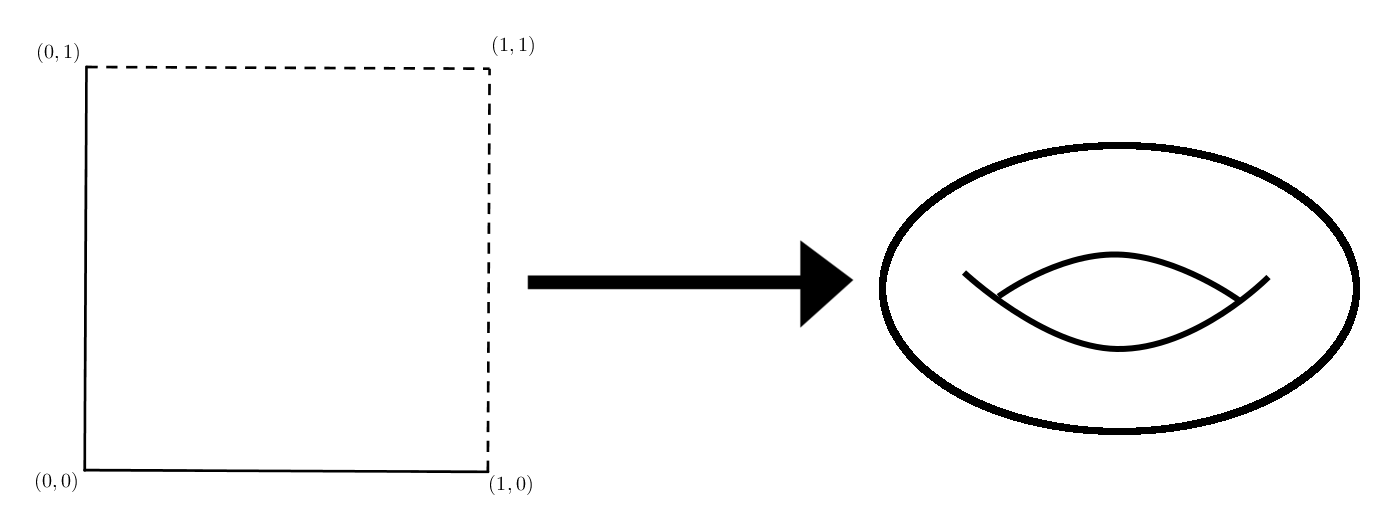
\includegraphics[width=0.7\linewidth]{images/frtorus}
	\caption{}
	\label{fig:frtorus}
\end{figure}

	

	
	

Open sets in the torus $\mathbb{R}$ are $\emptyset$ and $\mathbb{T}$, and the intersection of any standard open set with the fundamental region.  This is the same as the inherited subspace topology from $\mathbb{R}^2$.

\example{If we consider $\mathbb{R}^2/\mathbb{Z}$, where $a\in \mathbb{Z}$ acts on $\mathbb{R}^2$ by $a.(x,y)=(x+a,y)$.  A fundamental domain of this action is a vertical strip of unit width.  Again this inherits a subspace topology from $\mathbb{R}^2$.}



	







	\begin{figure}[!htb]
		\centering
		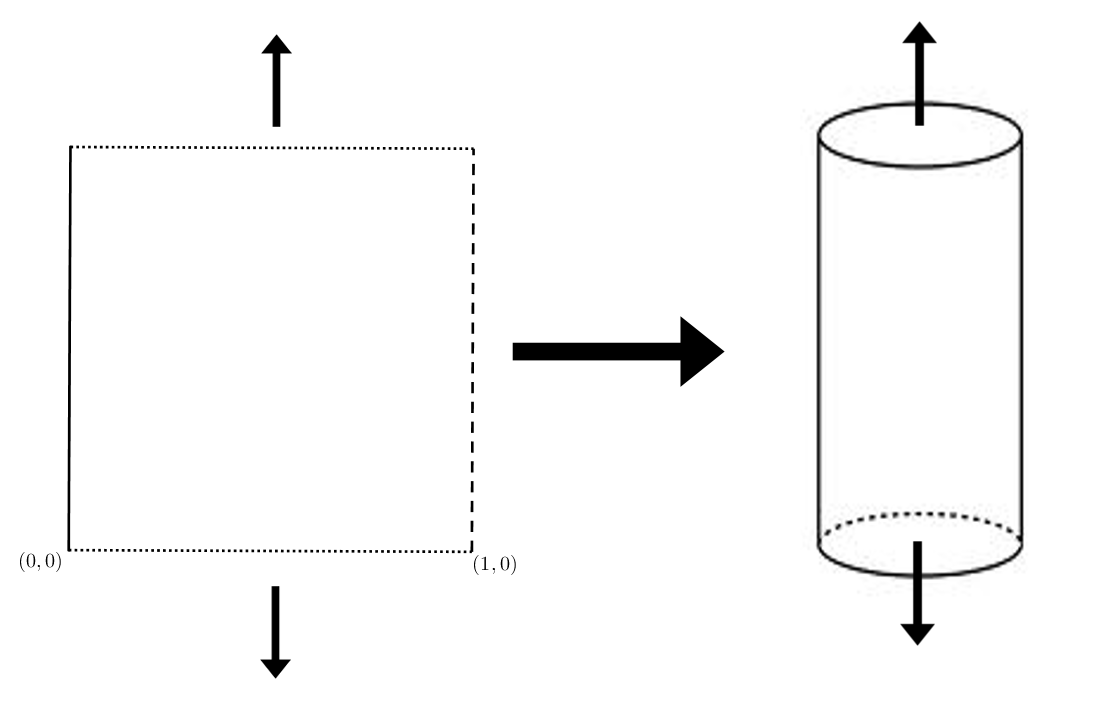
\includegraphics[width=0.7\linewidth]{images/frcyl}
		\caption{}
		\label{fig:frcyl}
	\end{figure}
	
	
	
	
	
\example{Consider again $\mathbb{R}^2/\mathbb{Z}$ but this time with the group action $a.(x,y)=(x+a,(-1)^ay)$.  The fundamental region is still a strip of unit width, but this time instead of identifying points on
	the boundary with their horizontal translation, we identify them with their horizontal translation
	composed with reflection about the $x$-axis. This space is homeomorphic to an infinite Moebius strip,
	which is difficult to draw.}


\example{Consider the equivalence relation on $\mathbb{R}^2$ described by $(x,y)\sim (x,y)$, $(0,y)\sim(1,y)$, and $(x,0)\sim(1-x,1)$.  The fundamental region again is a square with the left and right edges identified
	by simple translation, but the top and bottom edges are now identified by translation plus a flip
	across the square’s vertical axis of symmetry. This is homeomorphic to the Klein bottle, which is,
	again, hard to draw.}

\example{The previous example where we also identify the left and right edges by translation and
	a flip is called the real projective plane, denoted $\mathbb{R}P^2$
	. Both vertical and horizontal strips of this
	space look like Moebius strips. This is, once again, not easy to draw.}

\example{This one we can draw! Take the unit square as the fundamental region, but identify
	the top and left edge with each other by symmetry about the corner where they intersect, and do
	the same for the bottom and right edge. This space is homeomporhic to the 2-sphere $\mathbb{S}^2$
	.}
	
	
\begin{figure}[!htb]
\centering
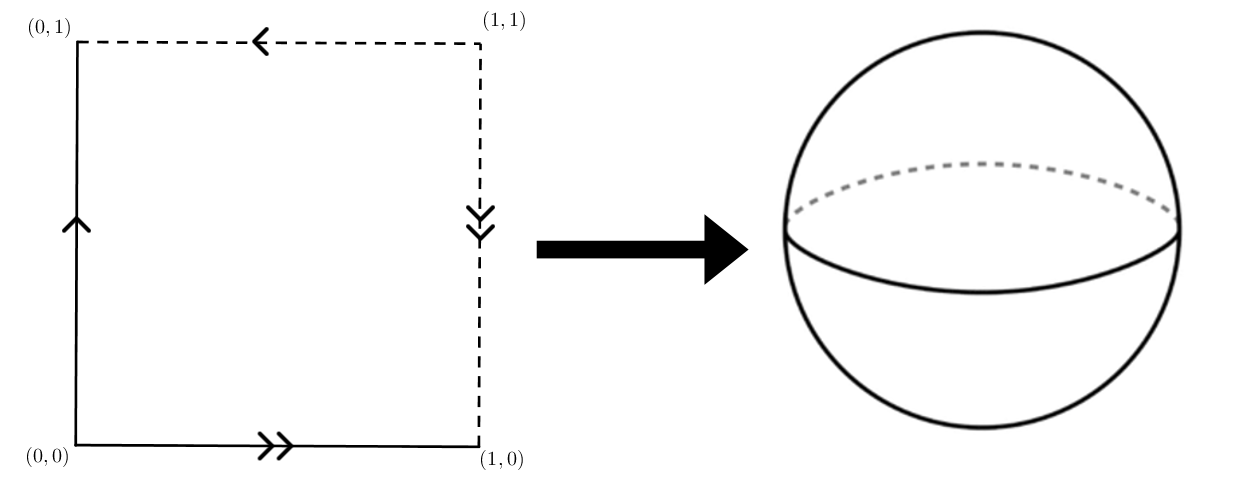
\includegraphics[width=0.7\linewidth]{images/frs2}
\caption{}
\label{fig:frs2}
\end{figure}
	
	
	
	


	\classheader{09-08-2017}


\section*{Mapping Cylinders and Tori}


\definition{Let $I$ denote the closed unit interval $[0,1]$.  The \textbf{mapping cylinder} of a continuous map $:fX\rightarrow Y$ is the quotient space defined by $X\times I/\sim$, where $(x,0)\sim (f(x),1)$.}


\definition{The \textbf{mapping torus} of a map $f:X\rightarrow X$ is similar, except that we require that the map be from a space to a copy of itself and we define the equivalence relation as $(x,0)\sim(f(x),0)$.}

\example{The mapping cylinder of $f:\mathbb{S}^1\rightarrow \mathbb{S}^1$ where $f(x)=x$ is a regular old cylinder.  The mapping torus is a regular old torus.}

\example{We can equivalently think of $\mathbb{S}^1$ as $\{ (x,y)|x^2+y^2=1 \}$ in Euclidean space or as $\{(r,\theta)|r=1  \}$ in polar coordinates.  Using this second formulation, consider the map $f:\mathbb{S}^1\rightarrow \mathbb{S}^1$ where $f(\theta)=2\theta$.  This is a two-to-one map which maps antipodal points to each other.  The mapping cylinder of $f$ is a Moebius strip.}

\example{What about the three-to-one map $f(\theta)=3\theta$?  The mapping cylinder of this looks like a three-bladed wing with a one-third twist and the ends glued together.}

\section*{Boundaries and Exteriors}

Let $(X,\mathcal{A})$ be a topological space and let $K\subseteq X$.

\definition{The \textbf{interior} of $K$ is the largest open subset contained in $K$.  That is, it is the union of all $U\subset K$ such that $U\in \mathcal{A}$.}

\definition{The \textbf{closure} of $K$ is the smallest closed subset containing $K$.  That is, it is the intersection of all $V\superset K$ such that $(X-V)\in \mathcal{A}$.}

\definition{The \textbf{boundary} of $K$ is the intersection of the closure of $K$ with the closure of the complement of $K$, that is $Bd(K) = \overline{K}\cap \overline{X-K}$.  If $K$ is open, then $Bd(K) = \overline{K}-K$.  If $K$ is closed, then $Bd(K)=\emptyset$.}


\example{Take $K = \mathbb{Q}\cap [0,1]\subset \mathbb{R}$ with the standard topology on $\mathbb{R}$.  The interior of this set is empty, as there is no open interval which doesn't contain an irrational number, so $\emptyset$ is the largest open subset in $K$.  The closure of $K$ is the entire interval $[0,1]$, as there is no smaller closed set which contains all of the rationals in that interval.  We also have that the boundary $Bd(K) = [0,1]$.}

\example{Take $K=\mathbb{R}-\{0\}$ with the Zariski topology on $\mathbb{R}$.  The interior of $K$ is $K$, as $K$ is open.  The closure of $K$ is all of $\mathbb{R}$, and the boundary is $\{0\}$.}

\definition{A point $x$ is a \textbf{limit point} of $K\subset X$ if every open set containing $x$ has non-empty intersection with $K$.  Equivalently, $x$ is a limit point of $K$ if $x\in \overline{K-\{x\}}$.}



\example{Take $\mathbb{R}$ with the Zariski topology.  If $U$ is an open set, then every $x\in\mathbb{R}$ is a limit point of $U$.  In fact, for any infinite subset of $\mathbb{R}$, every point in $\mathbb{R}$ is a limit point.}



	
	\classheader{09-11-2017}


\section*{Topological Bases}

\definition{Let $X$ be a set.  A collection $\mathcal{B}$ of subsets of $X$ is called a \textbf{base} (or \textbf{basis}) of $X$ if:
	
	\begin{enumerate}
		\item[1] If $x\in X$ then there is a $B\in \mathcal{B}$ such that $x\in B$.  Equivalently, $\mathcal{B}$ covers $X$.
		\item[2] If $B_1,B_2 \in \mathcal{B}$ and $x\in B_1\cap B_2$, then there is a $B_3\in\mathcal{B}$ such that $B_3\subset B_1\cap B_2$ and $x\in B_3$.
	\end{enumerate}
}

This is a weaker concept than a topology; we don't require that the union of base elements is a base element and we only require that the intersection of base elements contains another base element.

\example{Consider $\mathbb{R}^2$ with the standard topology.  Define $\mathcal{B} = \{ B_x(r) |x\in\mathbb{R}^2,r>0 \}$ as the set of open balls in $\mathbb{R}^2$. This is a base.  It is easy to see the first criterion is satisfied.  To see the second, consider two balls which both contain some point $x$.  Then there is a small ball centered at $x$ which is fully contained in the intersection of the two balls.  This smaller ball is also a base element, so we are done.}

\lemma{If $\mathcal{B}$ is a base and  $B_1,B_2,\dots,B_n \in \mathcal{B}$, and $x\in B_1\cap B_2\cap\dots\cap B_n$ then there exists a base element $B'\subset B_1\cap\dots\cap B_n$ which contains $x$.}

\begin{proof}
	We proceed by induction.  Since $x\in B_1\cap B_2$, there exists some $D_1\in\mathcal{B}$ such that $x\in D_1\subset B_1\cap B_2$.  Then $x\in D_1\cap B_3$, so there exists some $D_2\in\mathcal{B}$ with $x\in D_2$.  We proceed iteratively like this to find there is some $D_{n-1}\in \mathcal{B}$ with $x\in D_{n-1}$, and we set $B'=D_{n-1}$.
	
	
	
\end{proof}
	

\definition{A \textbf{topology generated by a base} is the collection of sets which are unions of base elements.}

If $X$ is a set with a base $\mathcal{B}$, then there is a smallest (coarsest) topology on $X$ containing $\mathcal{B}$, which is the topology generated by $\mathcal{B}$.  Open sets are the base elements, arbitrary unions of base elements, and $\emptyset$ and $X$ by definition.  Do we get the intersection property as well?

\claim{Yes.}

\begin{proof}
	If $B_1,\dots,B_n$ are base elements, then we can write the intersection $\bigcap\limits_{i\in [n]}B_i$ as the union of base elements just by taking neighborhoods of each point in the intersection.  If we have $U_1,\dots,U_n$ open in $X$ and $x\in \bigcap\limits_{i\in[n]}U_i$, then there is some base element in the intersection containing $x$.  If we do this for all points in the intersection, we can write the intersection as an arbitrary union of base elements, and we are done.
\end{proof}

\definition{Let $(X,\mathcal{A}$ be a topological space.  Take $\mathcal{B}\subset \mathcal{A}$ a collection of sets such that $\emptyset,X\in \mathcal{B}$ and if $x\in U\in \mathcal{A}$, then there is some $B\in\mathcal{B}$ such that $x\in B\subset U$.  We call $\mathcal{B}$ a \textbf{base for the topology $\boldsymbol{\mathcal{A}}$}.}


	\classheader{09-13-2017}



\section*{Bases, Separability, Hausdorff}

\definition{If $(X,\mathcal{A})$ is a topological space and $p$ a point in $X$, then a \textbf{base at the point $\boldsymbol{p}$} is a collection $\mathcal{U}$ of open sets such that whenever $p$ is in some $V\in \mathcal{A}$, there exists a $U\in\mathcal{U}$ with $p\in U\in\mathcal{U}$.}

\example{The set of open balls centered at $p$ form a base at $p$ in $\mathbb{R}^n$ with the standard topology.}

\example{The set of open balls forms a base for $\mathbb{R}^n$.  So does the set of all rectangular prisms.  So does the set of all cubes.  The set of cubes is obviously a subset of the set of prisms, but neither of these is a subset or a superset of the set of balls.  We can also have a base where we have balls/prisms/cubes with rational centers and rational radii/side lengths.  The cardinality of these bases is the same as the cardinality of $\mathbb{Q}$.}

\definition{If a set has a base which has cardinality in bijection with some subset of $\mathbb{N}$ or $\mathbb{Q}$, then it has a \textbf{countable base}.}

Which topologies have countable bases?  We have seen that $\mathbb{R}^n$ with the standard topology does.  How about $\mathbb{R}^n$ with the discrete topology?  The answer is no.  Since every singleton set is open in the discrete topology, any base must contain every singleton.  Since the number of singleton subsets of $\mathbb{R}$ is uncountable, there cannot be a countable base.

\definition{A subset is \textbf{dense} if every open set in the space contains some element of the subset.}

\definition{A space is \textbf{separable} if it has a countable, dense subset.}

If a set has a countable base, it is  separable, one countable, dense subset is just a single element from each base element.

Observe that any topology on a finite or countable set is separable, as the set of singletons is countable.

\definition{A topological space is \textbf{Hausdorff} if whenever we have two points $p,q\in X$ with $p\neq q$, there exist disjoint open sets such that $p$ belongs to one and $q$ belongs to the other.}

\example{$\mathbb{R}^n$ with the standard topology is separable.  If $p\neq q$, we can take small open balls around $p$ and $q$ with radius less than half the distance between them.  These balls are disjoint and open, so we are done.}


\example{The set $[-1,1]$ with the either-or topology is not Hausdorff.  If we take $p$ to be any non-zero point in $(-1,1)$ and $q=0$, then any open set containing zero must also contain $p$.}

\example{The Zariski topology is not Hausdorff (this is on the homework).}


\example{The line with a double point, defined as $\mathbb{R}\sqcup\mathbb{R}/\sim$ with $x\sim y$ if $x=y$ and $x,y\neq 0$ looks like the real line with two zeros, call them $0_1$ and $0_2$.  The open sets in this topology are the empty set, the whole space, and anything that kind of looks like a standard open set.  This space is not Hausdorff.  Any open set containing $0_1$ necessarily contains a neighborhood of $0_2$, and vice versa.  This space is separable, however.  Rational balls will form a countable base, for example.}



\theorem{If $\mathcal{A}$ is a topology on $X$ and $\mathcal{B}$ is a base for $\mathcal{A}$, then $\mathcal{B}$ is a base.}
	
	\begin{proof}
		
		Clearly we have $\emptyset, X\in \mathcal{B}$.  We only need to show that any point in the intersection of two base elements $B_1,B_2$ is in a third base element $B_3\subset B_1\cap B_2$.  We have $B_1\cap B_2$ open because $\mathcal{B}\subset\mathcal{A}$.  So by the definition of a topology, there must e a $B_3\in \mathcal{B}$ with $x\in B_3\subset B_1\cap B_2$, and we're done.
		
	\end{proof}
	

\theorem{If $\mathcal{B}$ is a base for a set $X$ and $\mathcal{A}$ is the topology generated by $\mathcal{B}$, then $\mathcal{B}$ is a base for the topology $\mathcal{A}$.}

\begin{proof}
	This proof is also straightforward.  If $B_1,B_2\in \mathcal{B}$ are basis elements, and we take an $x\in B_1\cap B_2$ then there is some $B_3\in\mathcal{B}$ with $x\in B_3\subset B_1\cap B_2$.  Since $\mathcal{B}$ generates $\mathcal{A}$, if $x$ is in some open set $U\in\mathcal{A}$, then it is in the union of some collection $\{B_i\}\subset \mathcal{B}$, so $x\in B_j$ for some $B_j\in\mathcal{B}$ with $B_j\subset U$, and we are done.
\end{proof}





\definition{A \textbf{subbase} (or subbasis) for a set $X$ is a collection $\mathcal{S}$ of sets such that $\bigcup\limits_{S\in\mathcal{S}} S=X$.}


	\classheader{09-18-2017}

\definition{A topological space $X$ is \textbf{first-countable} if there exists a countable base at every point $x\in X$.}

\definition{A topological space $X$ is \textbf{second-countable} if it has a countable base.}

\example{Consider $\mathbb{R}\sqcup\mathbb{R}/\sim$, where $x\sim y$ if $x=y$ and $x,y<1$.  This looks like the line but with two copies of the point $\{1\}$ and a second copy of every point greater than $1$.  This space is not Hausdorff.  If we take an open set at the first copy of $1$, it must intersect any open neighborhood of the other copy of $1$.}

\example{Consider $\mathbb{R}\sqcup\mathbb{R}/\sim$, where $x\sim y$ if $x=y$ and $x,y\leq1$. This looks like the line with one branch extending towards $-\infty$  and two branches extending towards $+\infty$ from $1$.  This space is Hausdorff.  If we take an open neighborhood around $1$, we can see that the inverse image is open only if that neighborhood contains pieces of all three branches, so it isn't possible to have an open set that contains $1+\epsilon_1$ for all $\epsilon_1>0$ on one branch without also having some small neighborhood which also contains $1+\epsilon_2$ for some $\epsilon_2>0$ on the second.}


\section*{Back to Subbases}

Recall that a subbase $\mathcal{S}$ of a set $X$ is a collection of subsets such that $\bigcup\mathcal{S}=X$.

\definition{If $\mathcal{S}$ is a subbase, then \textbf{the topology generated by $\boldsymbol{\mathcal{S}}$} is the set of all arbitrary unions and finite intersections of elements of $\mathcal{S}$.}

The proof that this is in fact a topology is trivial.

\definition{If $\mathcal{S}$ is a subbase, then a base $\mathcal{B}$ formed by the set of all finite intersections of elements of $\mathcal{S}$ plus the set $X$ itself is \textbf{the base generated by $\boldsymbol{\mathcal{S}}$}.}

Again, the proof that this is a proper base is trivial.

\definition{Let $(X,\mathcal{A}_1)$ and $(Y,\mathcal{A}_2)$ be topological spaces with respective bases $\mathcal{B}_1\subset X$ and $\mathcal{B}_2\subset Y$.  Then $X\times Y$ has  a topology called the \textbf{product topology} which is generated by a base $\mathcal{B}_3$ where $W\in \mathcal{B}_3$ if and only if $W=U\times V$ for some $U\in\mathcal{B}_1$ and $V\in\mathcal{B}_2$.  That is, base elements in the product topology are products of the base elements in the factor topologies.}


\example{Consider $\mathbb{R}\times\mathbb{R}$ and let $\mathcal{B}_1=\mathcal{B}_2=\{ (a,b)|-\infty\leq a<b\leq +\infty  \}$ be bases for $\mathbb{R}$ which consist of all open intervals.  Then the base for $\mathbb{R}^2$, $\mathcal{B}_3=\{(a,b)\times(c,d) |(a,b)\in\mathcal{B}_1,(c,d)\in\mathcal{B}_2  \}$ is the set of open rectangles in $\mathbb{R}^2$.  We showed last time (in the general case of prisms in $\mathbb{R}^n$) that this is indeed a base.}

\definition{Let $(X,\mathcal{A}_1)$ and $(Y,\mathcal{A}_2)$ be topological spaces with respective bases $\mathcal{B}_1\subset X$ and $\mathcal{B}_2\subset Y$.  The the subbase $\mathcal{S} = \{ U\times Y | U\in\mathcal{B}_1 \}\cup \{ X\times V|V\in\mathcal{B}_2 \}$ is the \textbf{standard subbase on $\boldsymbol{X\times Y}$}.}

The proof that the standard subbase generates the product topology extends naturally to all product topologies generated by a finite number of factor spaces.

We can think of the product of $k$ copies of $X$ as the set of functions from a set of size $k$ to $X$, $X^k = \{ f:[k]\rightarrow X\}$.

\example{We can think of $\mathbb{R}^3$ as $\{  f: \{1,2,3\}\rightarrow \mathbb{R} \}$.  $(f(1),f(2),f(3))$ is an ordered triple in $\mathbb{R}^3$, and it also completely specifies a function.  We can think of $\mathbb{R}^n$ as $\bigtimes\limits_{[n]}\mathbb{R}=\{ f:[n]\rightarrow\mathbb{R}\}$.  Similarly, the set of all functions from $\mathbb{R}$ to $\mathbb{R}$ is $\mathbb{R}^\mathbb{R}=\bigtimes\limits_\mathbb{R}\mathbb{R}$.}


	\classheader{09-20-2017}

\section*{The Cantor set}

The Cantor set is one of those pathological examples in mathematics.  Consider the interval $C_0=[0,1]\subset\mathbb{R}$.  Given $C_k$, define $C_{k+1}$ as $C_k$ with the middle third of each constituent interval removed.  So $$C_1=[0,\frac{1}{3}]\cup[\frac{2}{3},1]$$ $$C_2=[0,\frac{1}{9}]\cup[\frac{2}{9},\frac{1}{3}]\cup[\frac{2}{3},\frac{7}{9}]\cup[\frac{8}{9},1]$$ and so on.

While we don't have a precise definition for what it means to take a limit to $C_\infty$, we can define $C_\infty=\bigcap C_i$ and this is totally fine from a topological point of view.



\definition{The \textbf{Cantor set} is the name given to $C_\infty$.}

The Cantor set is not empty, it's actually uncountable.  To see this, consider all reals in $[0,1]$ expressed in their ternary expansion.  The Cantor set contains all numbers which do not have any $1$s in this representation.  This is obviously an uncountable set.  We also note that the Cantor set doesn't contain any intervals.  

The Cantor set inherits a subspace topology from $\mathbb{R}$.  It is an exercise on the homework to show that the map $f:C_\infty \rightarrow [0,1]$ where we replace all of the $2$s in the ternary representation with $1$s and interpret it as the binary representation of a real number is a continuous function.

The Cantor set has no interior points, so the complement of the Cantor set is dense and open.

\definition{Denote the \textbf{measure} of the set $C_k$ as $mC_k$. Here we'll use measure as `total length', although in a proper, measure-theoretic sense, this definition isn't quite correct.}

What is the measure of the Cantor set?  The measure of $C_0=[0,1]$ is $1$.  We can define a recurrence, where $mC_k=1-\frac{1}{2}\sum\limits_{i=1}^{k}(\frac{2}{3})^i$.  Then, $mC_\infty = 1-\frac{1}{2}\sum\limits_{i=1}^{\infty}(\frac{2}{3})^i = 1-\frac{1}{2}\frac{\frac{2}{3}}{1-\frac{2}{3}}=0$.

What if at each stage we remove a little less than $\frac{1}{3}$ of each interval?  Say we remove $\frac{\alpha}{3}$, where $0<\alpha<1$.  We still get a Cantor-like set, but here we get a recurrence which looks like $mC_k=mC_{k-1}-2^{k-1}\alpha(\frac{1}{3})^k$.  Here, the measure of $C_\infty$ is $1-\alpha$, but its interior is still empty, so its complement is open and dense.

We can even make a Cantor-like set of full measure by putting a smaller copy of the Cantor set into each gap created by removing an interval.  This set is uncountable, has measure $1$, and is nowhere dense.
	\classheader{09-22-2017}

\section*{Back To Bases}

How can we determine if two bases generate the same topology?

\begin{theorem}
	
	Let $\mathcal{A}$ and $\mathcal{A}'$ be two topologies on the same underlying set $X$ generated by bases $\mathcal{B}$ and $\mathcal{B}'$, respectively.  Then the following are equivalent:
	
	\begin{enumerate}
		\item $\mathcal{A}'$ is finer than $\mathcal{A}$
		\item If $x$ is in $X$ and $x$ is in some base element $B\in\mathcal{B}$, then there exists a $B'\in\mathcal{B}'$ such that $x\in B'$ and $B'\subset B$.
	\end{enumerate}
	
	
	
\end{theorem}

\begin{proof}
	
	Assume that $\mathcal{A}'$ is finer than $\mathcal{A}$ and take some $x\in X$ and some $B\in\mathcal{B}$ such that $x\in B$.  Since $B$ is an open set in $\mathcal{A}$, $B$ is also an open set in $\mathcal{A}'$, so $B$ can be written as the union $\bigcup B'_i$ for some $\{B'_i\}\subset \mathcal{B}'$.  Since $x\in B$, $x$ is in the union of these $B'_i$, so $x$ must be in at least one of the $B'_i$ which by construction is a subset of $B$.
	
	Now, assume that $x\in B\in\mathcal{B}$ implies the existence of some $B'\in\mathcal{B}'$ with $x\in B'\subset B$.  By taking intersections and small neighborhoods, we can necessarily write any such $B$ as a union of some collection of $B'_i$.  But since we can do this, any open set built from elements of $\mathcal{B}$ can be built from elements of $\mathcal{B}'$, so any open set in $\mathcal{A}$ is also open in $\mathcal{A}'$, hence $\mathcal{A}'$ is finer than $\mathcal{A}$.
	
	
	
\end{proof}

\section*{The Product Topology}

\remark{The book uses $\mathbb{R}^\omega$ to denote the set of all sequences in $\mathbb{R}$ indexed by the natural numbers and $\mathbb{R}^\infty$ to denote those sequences which are eventually all zeros.  We'll do our best to be consistent with this.}


\definition{Given a product of topological spaces $\prod X_\alpha$, the \textbf{box topology} is the one with open sets that can be written as a product $\prod U_\alpha$ where $U_alpha$ is open in $X_\alpha$.}

Under infinite products, this topology is too fine.  Consider the function $f:\mathbb{R}\rightarrow \mathbb{R}^\omega$, where $f(t)=(t,t,t,\dots)$.  This function is not continuous from the standard topology to the box topology. To see this, consider the set $(-1,1)\times (-\frac{1}{2},\frac{1}{2})\times (-\frac{-1}{3})\times \dots$ in $\mathbb{R}^\omega$.  This is open in the box topology.  Under $f$, the inverse image of this set is $\{0\}$, which is not open.

\definition{Let $\pi_\alpha(x)$ be the function which sends $x$ in the product to its $\alpha$ coordinate.  This extends to sets by saying that $\pi_\alpha(U)$ is the set of elements $y\in X_\alpha$ such that there exists some $x\in U$ where $\pi_\alpha(x) = y$.  The \textbf{product topology} is defined by the base consisting of the sets $\pi^{-1}_\alpha (U_\alpha)$ where $U_\alpha$ is a base element (or any open set) in $X_\alpha$.  Equivalently, an open set in the product topology is one which is a product of open sets in the factor spaces where all but finitely many are equal to the whole space.}
	\classheader{09-25-2017}

\section*{Metric Topologies}


\definition{A \textbf{metric} on a space $X$ is a function $d:X\times X\rightarrow R_+$ which satisfies:
	
	\begin{enumerate}
		\item $d(x,y)=0$ if and only if $x=y$ (positivity)
		\item $d(x,y) = d(y,x)$ for all $x,y$ (symmetry)
		\item $d(x,z)\leq d(x,y)+d(y,z)$ (triangle inequality)
	\end{enumerate}
	
}

\definition{If $X$ is a space with metric $d$, and $x\in X$, $r>0$, \textbf{the ball of radius $\boldsymbol{r}$ centered at $\boldsymbol{x}$} is the set $\{y|d(x,y)<r\}$.  This is denoted $B_r(x)$ (or $B_x(r)$, $B(x,r)$, $B(r,x)\dots$).}

\definition{The \textbf{topology generated by a metric} is the topology on a metric space generated by the base of all balls of finite radius centered at all points.}



If $x$ is an element of $X$ and $x$ is in some set $U$ which is open in the metric topology, then there is a sufficiently small $r$ such that $B_r(x)$ is entirely contained in $U$.  Hence all points of $U$ are interior.

Let's note that while such a base does indeed generate the topology we want, it's not always the best or smallest base that does so.  For example, the set of all balls of rational radius with rational center generates the standard topology on $\mathbb{R}^n$.

In fact, every metric space is at least first-countable, as we can take a base at a point consisting of the balls centered at that point of rational radius.

Metric spaces are also Hausdorff.  To  see this, consider two distinct points $x,y$.  Since they are not identical, the distance between them is positive, say $3\epsilon$.  Then $B_\epsilon(x)$ and $B_\epsilon(y)$ are disjoint open sets separating $x$ and $y$.

\definition{The \textbf{discrete metric} is the metric $d(x,y) = 0$ if $x=y$ and $1$ if $x\neq y$.}

\claim{The discrete metric generates the discrete topology.  }

\begin{proof}
	
To see this, consider the ball $B_{\frac{1}{2}}(x)$.  This is just the set $\{x\}$, and since the singletons are open, the corresponding topology must be the discrete one.
\end{proof}

\claim{The trivial topology is not generated by any metric.}

\begin{proof}
	The trivial topology is not Hausdorff, so it cannot be a metric topology.
\end{proof}


The Euclidean metric on $\mathbb{R}^n$, $d(x,y)=\sqrt{\sum(x_i-y_i)^2}$ generates the standard topology.

\definition{The \textbf{$\boldsymbol{\ell^p}$ metric} on $\mathbb{R}^n$ is $d(x,y) = \left(\sum|x_i-y_i|^p\right)^{\frac{1}{p}}$.}

\definition{The \textbf{$\boldsymbol{\ell^\infty}$ metric} on $\mathbb{R}^n$ is $d(x,y) = \sup\{|x_i-y_i|\}$.}

\claim{All of the $\ell^p$ metrics generate the same topology on $\mathbb{R}^n$.}

\begin{proof}
	Pick two metrics $\ell^p$ and $\ell^q$ with $p<q$.  We'll argue that base elements (balls) in one topology contain base elements of the other.  Containment one way is trivial.  For a fixed radius $r$, the $\ell^p$ ball of radius $r$ sits inside of the $\ell^q$ ball of radius $r$.  To see containment the other way, consider the $\ell^q$ ball of radius $r_1$ and think of it as an open set in the $\ell^p$ topology.  There is some point of maximum distance from the center, and if we pick some radius $r_2$ less than this, the ball will sit inside of the $\ell^q$ ball, and we're done.
\end{proof}


We call $\ell^p(\mathbb{R}^\omega)$ the set of sequences whose $\ell^p$ norm is finite.  This forms a vector space.
	\classheader{09-25-2017}

\section*{Metrics, Continued}

Recall that $\ell^p$ is a proper subset of $\mathbb{R}^\omega$.

\definition{The \textbf{$\boldsymbol{\ell^p}$ norm} on $\mathbb{R}^n$ is $d(x,y) = \left(\sum|x_i|^p\right)^{\frac{1}{p}}$.}

\definition{The \textbf{$\boldsymbol{\ell^\infty}$ norm} on $\mathbb{R}^n$ is $d(x,y) = \sup\{|x_i|\}$.}

If $X$ is a vector space, then a function $||\cdot ||: X\rightarrow \mathbb{R}$ is a norm if:

\begin{enumerate}
	\item $||\vec{x}||\geq 0$ for all $x\in X$ with equality if and only if $x=\vec{0}$
	\item $||c\vec{x}|| = |c|\cdot||\vec{x}||$ for all scalars $c$ and vectors $\vec{x}$
	\item $||\vec{x}+\vec{y}|| \leq ||\vec{x}||+||\vec{y}||$ for all vectors $\vec{x},\vec{y}$
\end{enumerate}

\definition{We call such an $X$ a \textbf{normed vector space}.}

Metrics do not need to come from norms, but norms induce metrics.  A normed vector space is a metric space, but a metric space need not be a normed vector space.

Consider the function $f:\mathbb{R}\rightarrow \mathbb{R}$ with a norm 
$$||f||_p = \left(\int_{-\infty}^{\infty}|f(x)|^p dx\right)^\frac{1}{p}$$

\definition{This is called the \textbf{$\boldsymbol{L^p}$ pseudonorm}.}

Why is this a pseudonorm?  There are functions which are non-zero which have zero integral, such as functions which are zero everywhere except on a set of measure zero.  We can resolve this by defining an equivalence relation $\sim$ where $f\sim g$ if and only if $||f-g||_p=0$.  These equivalence classes form the vector space of $L^p$ functions on $\mathbb{R}$, denoted $L^p(\mathbb{R})$.  On these classes, the $L^p$ pseudonorm $||\cdot ||_p$ is a proper norm.  As it turns out, these are actually \textit{complete} normed vector spaces, i.e. Banach spaces.

\definition{Given a metric $d(x,y)$, we can create a \textbf{bounded metric} $\bar{d}(x,y)$ by defining $\bar{d}(x,y)=\min(d(x,y),1)$.  It is easy to see that this forms a proper metric.}

When do two metrics generate the same topology?  Metric balls form a base.  If we can show that balls in one metric contain balls in the other, and vice versa, then the metrics generate the same topology.

\definition{The \textbf{Hilbert cube} is the set $I^\omega \subset \mathbb{R}^\omega$.  That is, it is the set of all sequences with entries from the interval $[0,1]$.}

The Hilbert cube has finite volume, but the diagonal has infinite length.  That is, the point $(0,0,0,\dots)$ is infinitely far from the point $(1,1,1,\dots)$ with respect to any $\ell^p$ metric (for finite $p$).  This space is homeomorphic to the ball of radius $1$ in the $\ell^\infty$ metric.

A subbase for the Hilbert cube is the set $\{ \pi_i^{-1}(U) | U \ open \ in \ [0,1] \}$.

\definition{A topological space is \textbf{metrizable} if there exists a metric on $X$ which generates that topology.}

As an example, the standard topology on $\mathbb{R}^n$ is metrizable as it is generated by the $\ell^2$ metric, for example.

Since metric spaces are first-countable, first-countability is a necessary condition for a space to be metrizable.

\example{$\mathbb{R}^\mathbb{R}$ with the product topology is not first-countable, therefore there does not exist a metric on $\mathbb{R}^\mathbb{R}$ which generates the product topology.}

\theorem{A countable product of metric spaces (with the product topology) is metrizable.}

\begin{proof}
	
	Let $X$ be a metric space with metric $d$ and consider the product $X^\mathbb{N}$.  Let $x=(x_1,x_2,\dots)$ and $y=(y_1,y_2,\dots)$ be points in $X^\mathbb{N}$.  Next, define $D(x,y) = \sup\left\{\frac{\bar{d}(x_i,y_i)}{i}\right\}$ where $\bar{d}$ is the bounded version of $d$.  It's easy to see that $D$ is a proper metric.
	
	Under $D$, the ball of radius $r$ centered at $x$ is 
	
\begin{align*}
B_r(x) &= \{ y\in X^\mathbb{N} | D(x,y)<r   \}\\
\ \\
&= \left\{  y\in X^\mathbb{N} | \bar{d}(x_1,y_1) < r ,\ \bar{d}(x_2,y_2) < 2r, \ \bar{d}(x_3,y_3)<3r,\dots              \right\}
\end{align*}
	
Since eventually $nr$ becomes larger than $1$, everything beyond the $n$th point must be inside the ball.  Thus, only finitely many $(x_i,y_i)$ need to be checked, so these balls look like the product of finitely many open balls in $X$ and infinitely many copies of $X$ itself, which is a base for the product topology.
	
\end{proof}
	\classheader{09-29-2017}

\section*{Metrics, Continued, Continued}
\subsection*{The Fourier Transform}

If $D\subset \R^n$ is open, we can define $L^p(D)=\left\{  f:D\rightarrow\R |\left( \int_D |f(x)|^p dx\right)^\frac{1}{p}  < \infty   \right\}/{\sim}$, the set of functions whose $L^p$ norm over $D$ is finite modulo the usual equivalence relation where $f$ and $g$ are equivalent if the $L^p$ integral of $f-g$ is zero.

Recall the definitions of $\ell^p$ and $\ell^\infty$,
$$\ell^p = \left\{ (x_1,x_2,\dots) | \left(\sum|x_i|^p\right)^\frac{1}{p} < \infty \right\}$$
$$\ell^\infty = \left\{ (x_1,x_2,\dots) | \sup|x_i| < \infty \right\}$$

the set of sequences in $\R$ with bounded $p$-norm and bounded maximal element, respectively.

These $\ell^p$ spaces are normed vector spaces (actually, metric spaces).  We'll take this on faith because it's not difficult, but rather time consuming, to prove the triangle inequality holds here.
\definition{The \textbf{Fourier Transform} is defined as the following:

Let $I$ denote the closed interval $[-1,1]$, and consider $L^2(I)$, the set of square-integrable functions (modulo equivalence) on $I$.  If a function $f\in L^2(I)$, then we can write 
$$f(x) = \sum\limits_{n=-\infty}^{\infty} a_ne^{i\pi n x}$$
and
$$a_n = \int_{-1}^{1} f(x)e^{i\pi n x}dx$$

}

This defines a map $\mathscr{F}:L^2(I)\rightarrow \R^\infty$ where $f\xmapsto[]{\mathscr{F}}(\dots ,a_{-2},a_{-1},a_0,a_1,a_2,\dots)$.  It turns out that $\mathscr{F}$ is an injective linear map.  Parseval's Theorem states that if $f\in L^2(I)$ and $\{a_i\}_1^\infty \in \mathbb{R}^\infty$, is the Fourier transform of $f$, then 

$$\left(\int_I |f(x)|^2 dx \right)^\frac{1}{2} = \left(\sum\limits_{-\infty}^\infty |a_n|^2\right)^\frac{1}{2}$$

Thus $\mathscr{F}$ is an isometric linear injection.  We can also show surjectivity by reversing the construction, so $\mathscr{F}$ defines an isometric isomorphism between $\ell^2$ and $L^2(I)$.

\section*{Convergent Sequences}

\definition{If $X$ is a set, then a \textbf{sequence} of points in $X$ is an ordered list $(x_1,x_2,x_3,\dots)$ such that each $x_i\in X$.}

\definition{A point $x\in X$ is a \textbf{cluster point} of a sequence $S = (x_1,x_2,\dots)$ if $x\in \bigcap\limits_{N=1}^\infty\overline{\bigcup\limits_{i\geq N} \left\{x_i\right\}}$. That is, $x$ is in the closure of every tail of $S$.
	}
	
\definition{A point $x\in X$ is a \textbf{limit point} of $S=(x_1,x_2,\dots)$ if $x\in \bigcap\limits_{n\subset \mathbb{N}}\overline{\bigcup\limits_{i\in n}\left\{ x_i\right\}}$ where $n\subset \mathbb{N}$ is infinite.  That is, $x$ is a limit point if all infinite subsequences of $S$ have $x$ in their closure.}


\example{Take $S=(1,-1,1,-1,\dots)$ to be a sequence in $\R$.  Every tail of this sequence have all elements in $\left\{ -1,1  \right\}$, and this is just its own closure, so the cluster points are $-1$ and $1$.  This sequence has no limit points, however.  We can pick infinite subsequences which look like $(1,1,1,\dots)$ and $(-1,-1,-1,\dots)$, and $(-1,1,-1,1,\dots)$, and the intersection of the sets $\{-1\}\cap \{1\},\cap \{-1,1\}$ is empty.}

\example{Consider the line with a double point, $\R-\{0\}\cup \{0_1,0_2\}$ and the sequence $S=(1,\frac{1}{2},\frac{1}{3},\dots)$.  The limit points of $S$ are $0_1$ and $0_2$.  To see this, observe that every open set around either $0_1$ or $0_2$ contains infinitely many points in the sequence, hence $0_1$ and $0_2$ are both in the closure of the intersection of all infinite subsequences.}

\theorem{If a topological space $X$ is Hausdorff, then the set of limit points of any sequence of points in $X$ has at most one element.}

\begin{proof}
	Suppose, for the sake of contradiction, that $X$ is Hausdorff and $x\neq y$ are both limits of a sequence $S=(x_1,x_2,x_3,\dots)$.  Since $X$ is Hausdorff, we can find disjoint open sets $U_x$ and $U_y$ which separate $x$ and $y$.  Since $x$ and $y$ are limit points and $U_x$ and $U_y$ are neighborhoods of $x$ and $y$, infinitely many points of the sequence lie in both $U_x$ and $U_y$.  Since we assumed that the set of limit points is non-empty, this implies the intersection of $U_x$ and $U_y$ is non-empty, contradicting the assumption that they are disjoint.  Hence a sequence cannot have more than one limit point in a Hausdorff space.
\end{proof}

\definition{Given $A\subseteq X$, a point $x$ is in the \textbf{sequential closure} of $A$ if there exists a sequence $S$ in $A$ such that $x$ is a limit point of $S$.}

\thrm{If $x$ is in the sequential closure of $A\subseteq X$, then $x\in \overline{A}$.  The converse is true if we add the condition that $X$ is first-countable, but we will not show this now.}

\begin{proof}
	Take $A\subseteq X$ and $S$ a sequence in $A$, and assume that $x$ is a limit point of $S$.  Then by definition, $x\in \overline{\bigcup\limits_{x_i \in T} \{x_i\}}$ for some subsequence $T$.  So $x\in \overline{\bigcup\limits_{x_i \in T} \{x_i\}} \subset\overline{\bigcup\limits_{x \in A} \{x\}} = \overline{A}$, and we are done.
\end{proof}
	\classheader{10-02-2017}

\section*{Topological Groups}

We will look at some topological properties of matrix groups.  Throughout, we will assume everything happens with respect to some fixed basis.

\definition{The group $\boldsymbol{O(n)}$ is the set of rigid transformations of $n$-dimensional Euclidean space which leaves the origin fixed.  That is, $A\in O(n)$ if and only if for any $\vec{x},\vec{y}\in\mathbb{R}^n$, $\innprod{\vec{x}}{\vec{y}} = \innprod{A\vec{x}}{A\vec{y}}$, where $\innprod{\cdot}{\cdot}$ is the standard Euclidean inner product.}

These matrices all have determinant $\pm 1$, and this holds with respect to every basis.

\definition{The group $\boldsymbol{SO(n)}$ is the subset of $O(n)$ of $n\times n$ matrices with determinant $+1$.}

We'll observe that $O(1) = \{-1,1\} = C_2$ and  $SO(1) = \{1\}$ is the trivial group.

$SO(2)$ is infinite, and can be thought of as the set of $2\times 2$ rotation matrices
$SO(2)= \left\{  \begin{pmatrix}
\cos\theta & -\sin\theta \\
\sin\theta & \cos\theta
\end{pmatrix}  | \theta\in\R   \right\}$

\definition{A \textbf{topological group}  $X$ is a set $X$ with a topology and a group structure such that the group operation $\circ :X\times X\rightarrow X$ is a continuous function.}

Topologically, we can think of $SO(2)$ as the unit circle in $\mathbb{R}^4$.

The group $SO(3)$ is harder to write down, but it is the set of $3\times 3$ matrices with determinant $1$ (equivalently, the $3x3$ matrices $A$ such that $AA^T=I$).

$SO(3)$ is generated by three one-parameter subgroups, which are copies of $SO(2)$ each fixing a dimension: 

$X_\theta = 
\begin{pmatrix} 
1 & 0 & 0 \\
0 & \cos\theta & -\sin\theta \\
0 & \sin\theta & \cos\theta
\end{pmatrix}
$ corresponds to rotation about the $x$-axis

$Y_\theta = 
\begin{pmatrix} 
\cos\theta & 0 & -\sin\theta \\
0 & 1 & 0 \\
\sin\theta & 0 &  \cos\theta
\end{pmatrix}
$ corresponds to rotation about the $y$-axis


$Z_\theta = 
\begin{pmatrix} 
\cos\theta  & -\sin\theta & 0 \\
\sin\theta &  \cos\theta & 0\\
0 & 0 & 1
\end{pmatrix}
$ corresponds to rotation about the $z$-axis

thus $SO(3) = \left\{  X_{\theta_1}\cdot Y_{\theta_2}\cdot Z_{\theta_3} | \theta_1,\theta_2,\theta_3\in \R  \right\}\subset \R^9$.

Since multiplication in $\R^9$ is a continuous function, matrix multiplication in $SO(3)$ is as well, so it is a topological group as well.  There is a homeomorphism between $SO(3)$ and $\R P^3$, the real projective plane of dimension $3$.  Thus, $SO(3)\simeq S^3/{\text{antipodal map}}$

\section*{Back to Sequences}

\lemma{The Sequence Lemma: If $A\subset X$ and $(x_1,x_2,x_3\dots)$ is a sequence in $A$ with $x$ as a limit point, then $x\in\overline{A}$ (we proved this last time).  Additionally, if $X$ is a first-countable space and $A\subset X$, then $x\in\overline{A}$ implies there exists a sequence in $A$ with $x$ as a limit point.}

\begin{proof}
	
	
	Let $\{B_i\}$ be a countable basis at $x$.  Because $x\in A$, we have that $B_i\cap A\neq \emptyset$, so there is at least one point in $B_i\cap A$ for all $B_i$.  For each, take one such point.  This defines a sequence $(x_1,x_2,x_3,\dots)$ in $A$.  By the definition of convergence, a sequence converges to $x$ of $x$ is in the closure of every subsequence.
	
    Take $U$ to be an open set containing $x$.  Then there exists some base element $B_N \subset U$ but by construction, $x_i\in B_N$ for all $i\geq N$, so $B_N$ contains every infinite subsequence, so $U$ also does.  Since $U$ is an open set around $x$ which has infinite intersection with any subsequence, $x$ is a limit point of the sequence.
	
	
	
\end{proof}

\definition{A function $f:X\rightarrow Y$ is \textbf{sequentially continuous} if whenever $S=(x_1,x_2,x_3,\dots)$ is a sequence in $X$ and $x$ is a limit point of $S$, then the sequence $T=(f(x_1),f(x_2),f(x_3),\dots)$ has (at least) $f(x)$ as a limit point.}

\thrm{If $f:X\rightarrow Y$ is continuous, then $f$ is sequentially continuous.}

\begin{proof}
	
	Take $S=(x_1,x_2,x_3,\dots)$ to be a sequence in $X$ with limit point $x$ and let $y=f(x)$.  Take $U$ to be an open neighborhood of $y$ in $Y$.
	
	By continuity, $f^{-1}(U)$ is an open neighborhood of $x$, and since $x$ is a limit point of $S$, the tails of all subsequences of $S$ are in $f^{-1}(U)$, so the image of the tails of all subsequences is in the image $U$.  Therefore, $y$ is a limit point of the sequence $(f(x_1),f(x_2),f(x_3),\dots)$, as desired.
	
	
	
\end{proof}
\corollary{By this theorem and the Sequence Lemma, we have that if $X$ is first-countable, then sequential continuity implies continuity.}

\corollary{In a metric space, continuity, sequential continuity, and $\epsilon-\delta$ continuity are all equivalent.}
	\classheader{10-04-2017}


\section*{More Topological Groups}

We have from before that $SO(3)\simeq \R P^3 \simeq \mathbb{S}^3/{\text{antipodal map}}$.


\definition{The groups $\boldsymbol{U(n),SU(n)}$ are defined analogously to $O(n)$ and $SO(n)$, except that these are rigid transformations of complex space $\mathbb{C}^n$. In $\mathbb{C}^n$, we define rigidity with respect to the Hermitian inner product $\innprod{\vec{v}}{\vec{w}} = \vec{v}^T\overline{\vec{w}}$.}

$SU(n)$ is the subset of $U(n)$ with determinant $1$.

We have that $SO(2)\simeq \mathbb{S}^1$, but also that $U(1) = \left\{  e^{i\theta}|\theta\in\R     \right\} \simeq \mathbb{S}^2$.  This leads to a natural group homomorphism and topological homeomorphism $e^{i\theta}\mapsto
 \begin{pmatrix} 
 \cos\theta & -\sin\theta\\
 \sin\theta & \cos\theta
 \end{pmatrix}$
 
 With a little bit of work, we can show that $SU(2)\simeq \mathbb{S}^3$.
 
 

\section*{Back to Continuity}

For the next section, we'll find the following characterization of continuity useful.

\thrm{The following are equivalent:
	Let $f:X\rightarrow Y$ be a function. Then $f$ is continuous if and only if:
	\begin{enumerate}
		\item $f^{-1}(U)\subset X$ is open whenever $U\subset Y$ is open.
		\item $f^{-1}(K)\subset X$ is closed whenever $K\subset Y$ is closed.
		\item $f(\overline{A}) \subset \overline{f(A)}$ for any $A\subset X$.
		
		
	\end{enumerate}
}
\begin{proof}
	
The first is our ordinary characterization of continuity and showing equivalence to the second is a simple exercise in taking set complements.  We'll use these to show that $f$ is continuous if and only if $f(\overline{A}) \subset \overline{f(A)}$ for any $A\subset X$.

Take $y\in f(\overline{A})$.  Suppose, for the sake of contradiction, that $y\notin \overline{f(A)}$, there exists an open set $U_y$ such that $y\in U_y$ and $U_y \cap f(A) = \emptyset$.  But we have that $f^{-1}(U_y)$ is an open set in $X$, and it intersects $A$ non-trivially, as in particular $A$ and $f^{-1}(U_y)$ both contain an $x$ such that $f(x)=y$.  Therefore $y\in \overline{f(A)}$, contradicting our assumption.

Now, suppose that $f(\overline{A})\subseteq \overline{f(A)}$, and take $K\subset Y$ to be closed.  We will show that $f^{-1}(K)$ must be closed, meaning $f$ is continuous.  Let $A=f^{-1}(K)$.  Then we have $f(\overline{A})\subset\overline{f(A)}$ by assumption, and by definition, $\overline{f(A)}=\overline{f(f^{-1}(K))}=\overline{K} = K$, since $K$ is closed.  Additionally, $f(\overline{f^{-1}(K)})\subseteq K$.  If $x\in \overline{f^{-1}(K)}$, then $f(x)\in K$, so $x\in f^{-1}(K)$ and because $\overline{f^{-1}(K)}=f^{-1}(K)$, we have that inverse images are closed, and we are done.
	
\end{proof}

\thrm{If $f:X\rightarrow Y$ is sequentially continuous and $X$ is first-countable, then $f$ is continuous.}

\begin{proof}
	
	Take $A\subset X$.  Since $X$ is first-countable, the sequential closure of $A$ is $\overline A$.  Take $x\in A$.  Then there exists a sequence $S=(x_1,x_2,x_3,\dots)$ in $A$ such that $x$ is a limit point of $S$.
	
	Since $f$ is sequentially continuous, $y=f(x)$ is a limit point of the sequence $(f(x_1),f(x_2),f(x_3),\dots)$.  But this is a sequence in $f(A)$, and since $x$ is in the sequential closure, and therefore the closure of $A$, $y$ is in the closure of $f(A)$.  Thus $f(\overline{A})\subseteq \overline{(f(A))}$, and we are done.

	
	
	
\end{proof}





	
	
	\classheader{10-06-2017}


\section*{The Order Topology}

Given an ordered set $X$ with a binary relation $<$ such that for all $x,y,z\in X$ with $x\neq y$, we have that

\begin{enumerate}
	\item $x\not < x$
	\item $x < y$ or $y<x$
	\item If $x<y$ and $y<z$, then $x<z$
	
	
\end{enumerate}

\definition{The \textbf{order topology} on $X$ is defined to be the topology generated by the base of all open intervals. That is, if $a<b$, then $\left\{  x | a<x<b   \right\}$ is a base element.}

We'll observe that in $\R$, this is the standard topology.

\definition{If $X$ is an ordered set and $Y=\prod\limits_1^n X_i$ is a finite product of copies of $X$, then $Y$ inherits an ordering called the \textbf{dictionary} or \textbf{lexicographic order}, where $(x_1,x_2,x_3,\dots,x_n) < (y_1,y_2,y_3,\dots,y_n)$ if and only if $x_i=y_i$ in the first $k-1$ positions and $x_k<y_k$.}

In $\R^2$ with the order topology, open sets looks like open vertical strips with two open rays adjoined


\begin{figure}[!htb]
	\centering
	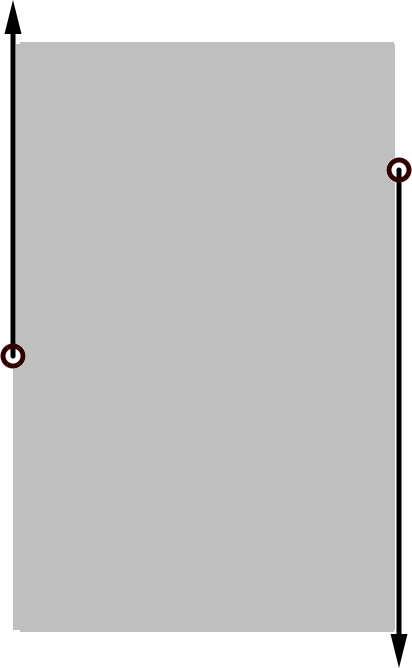
\includegraphics[scale=.2]{images/ordertopr2}
	\caption{An example of an open interval in the order topology on $\R^2$}
	\label{fig:ordtopr2}
\end{figure}

\section*{Convergence in Uncountable Product Spaces}

On $\R^I$, the set of functions $I\rightarrow \R$, we have three topologies: the product, the uniform, and the box topologies.  We also have that while the uniform topology is metrizable (clearly, as it comes from a metric), the box and product topologies are not.

Given a sequence $\left\{f_i\right\}\subset \mathbb{R}^I$:

The sequence $\left\{f_i\right\}$ converges in the product topology if and only if it converges pointwise.

The sequence $\left\{f_i\right\}$ converges in the uniform topology if and only if it converges uniformly, in the analytic sense.  That is, given $\epsilon>0$, there exists an $n\in\mathbb{N}$ such that for all $i>n$, $|f_i(x)-f(x)|< \epsilon$ everywhere.

The sequence $\left\{f_i\right\}$ converges in the box topology if and only if it converges pointwise and there exists an $n\in \mathbb{N}$ such that for all $i>n$, $f_i$ is constant everywhere except a finite set.


\thrm{(Weierstrass) If $\left\{f_i\right\}$ is a sequence of continuous functions which converges to a function $f$ in the uniform topology, then the limit $f$ is also a continuous function.}

\begin{proof}
	
	Take $x,y\in I$, and look at $|f(x)-f(y)|$.  Let $\epsilon>0$ be given.  By the triangle inequality, $|f(x)-f(y)| \leq |f_i(x)-f(x)| + |f_i(x)-f_i(y)|+|f_i(y)-f(y)|$.  By uniform convergence, there exists an $n\in\mathbb{N}$ such that $|f_i(x) - f(x)|$ and $|f_i(y)-f(y)|$ are each less than $\frac{\epsilon}{3}$.  Since each $f_i$ is continuous, there exists a $\delta >0$ such that $|x-y| < \delta$ implies $|f_n(x)-f_n(y)|<\frac{\epsilon}{3}$.  
	
	Thus, whenever $|x-y|<\delta$, we have that $|f(x)-f(y)| \leq |f_n(x)-f(x)| + |f_n(x)-f_n(y)|+|f_n(y)-f(y)| \leq \frac{\epsilon}{3} +\frac{\epsilon}{3} +\frac{\epsilon}{3} = \epsilon$, hence $f$ is continuous.
	
	\end{proof}
	
	
	
\definition{A topological space is \textbf{connected} if it cannot be written as the union of two (non-empty) disjoint open sets.}

\definition{A topological space is \textbf{disconnected} if there exist open sets $A,B$ such that $X=A\cup B$ and $A\cap B=\emptyset$.}



\thrm{A topological space $X$ is connected if and only if $\emptyset$ and $X$ are the only sets which are both closed and open in $X$.}

\begin{proof}
	
	If there exists some non-empty set $K$ which is both open and closed, the the complement of $K$ is also both closed and open, so $X=K\cup X-K$ is a way to write $X$ as the union of two disjoint open sets.  Thus $X$ is connected if and only if the only such $K$ is $X$ itself.
	
	
	\end{proof}


\definition{A \textbf{connected component} of a topological space $X$ is a set which is both closed and open in $X$.}

A topological space can be decomposed into connected components.

\thrm{Let $\sim$ denote the relation $x\sim y$ if and only if there is a connected open set $U$ containing $x$ and $y$.  Then $\sim$ is a proper equivalence relation and the set $\left\{ x | x\sim y \right\}$ is an equivalent characterization of the connected component of $y$.}

\corollary{If the above equivalence relation partitions $X$ into exactly one class, $X$ is connected.}

\definition{A topological space $X$ is \textbf{path connected} if for all $x,y\in X$ there exists a continuous function $p:[0,1]\rightarrow X$ such that $p(0)=x$ and $p(1)=y$.}

We can do a similar thing as above to describe path connected components with an equivalence relation.


	
	\classheader{10-09-2017}

\definition{A topological space $X$ is \textbf{locally connected} at $x$ if every open set $U$ containing $x$ has the property that there exists a $V\subseteq U$ such that $x\in V$, $V$ is open, and $V$ is connected.}

\definition{A topological space is \textbf{locally path connected} at $x$ if every open set $U$ containing $x$ has the property that there exists a $V\subseteq U$ such that $x\in V$, $V$ is open, and $V$ is path connected.}

\example{The topologist's interval is the subset of $\R^2$ defined piecewise as the union of the closed horizontal segment $[-1,0]$ along the $x$-axis, the closed vertical segment $[-1,1]$ along the $y$-axis, and the function $y=\sin(\frac{\pi}{x})$ on the interval $x\in (0,1]$. We give this the subspace topology from $\R^2$.
	
	
	\begin{figure}[!htb]
		\centering
		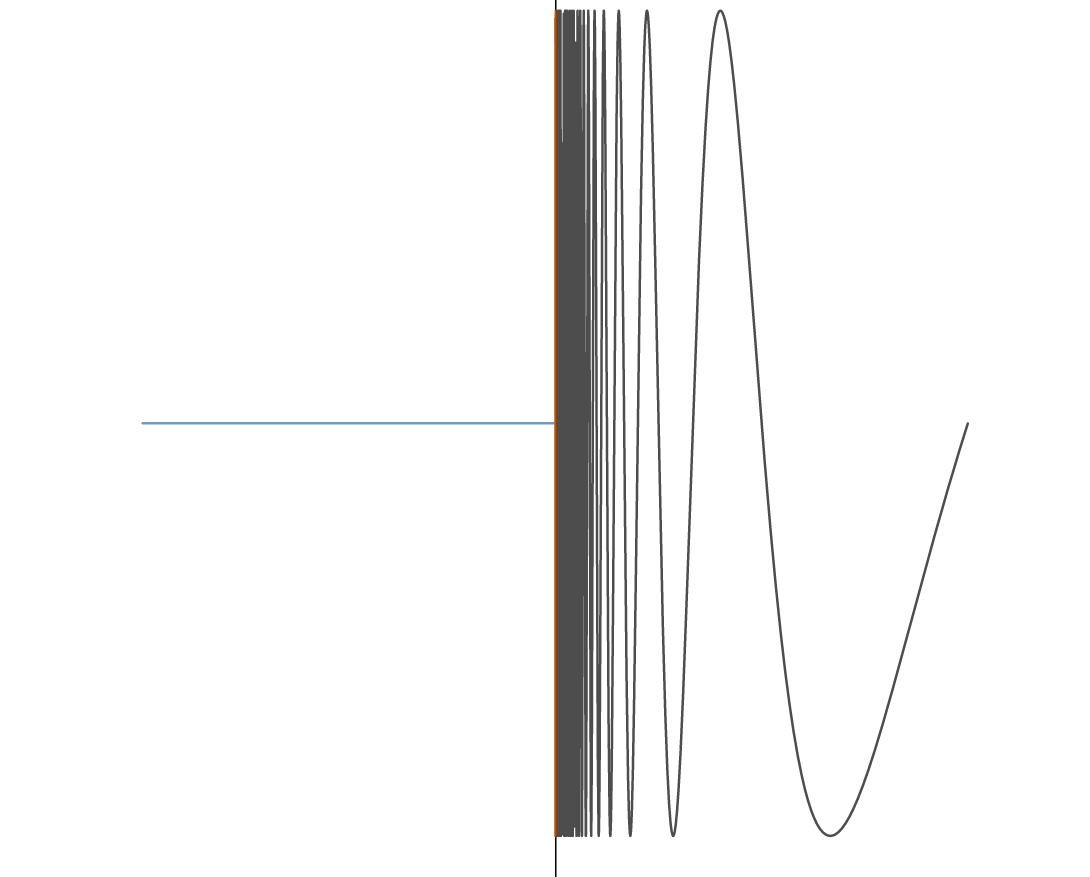
\includegraphics[scale=.2]{images/topint}
		\caption{The Topologist's Interval}
		\label{fig:topint}
	\end{figure}
	
	
	This space is connected, but not path connected, as the vertical stripes become infinitely close near zero, so there is no proper path from a point to the left of the origin to a point to the right.
	
	
	The topologist's circle is the same thing, but with an arc adjoined from $(1,0)$ to $(-1,0)$.
	
	\begin{figure}[!htb]
		\centering
		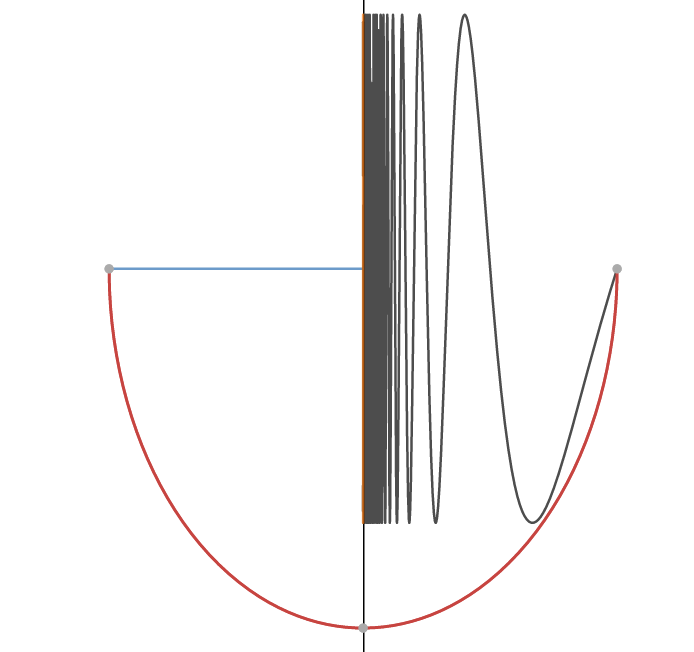
\includegraphics[scale=.3]{images/topcirc}
		\caption{The Topologist's Circle}
		\label{fig:topcirc}
	\end{figure}
	
	This space is connected and path connected, as we can use the arc to avoid the messiness to the right of the origin, but it is not locally path connected, as we can still look at small neighborhoods which look like parallel stripes, and obviously are not path connected.



The subset of $\R^2$ defined piecewise as the union of the closed horizontal segment $[-1,0]$ along the $x$-axis and $y=x\sin(\frac{\pi}{x})$ is locally connected everywhere, but not locally path connected at the origin.


	
	\begin{figure}[!htb]
		\centering
		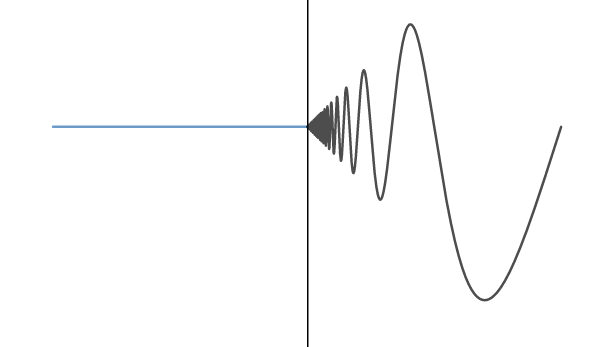
\includegraphics[scale=.3]{images/xsinx}
		\caption{$y=x\sin{\pi/x}$}
		\label{fig:xsinx}
	\end{figure}

}

\thrm{If a space $X$ is path connected, then it is connected.}

\begin{proof}
	
	Let $X$ be a path connected topological space.  If $X$ is not connected, then there exist open sets $A$ and $B$ such that $A\cup B=X$, so if we picked an $x\in A$ and $y\in B$, then the path between them would be split.  If $p$ is our path function, then one of $p^{-1}(A)$ or $p^{-1}(B)$ is the closed interval $[0,a]$ or $[b,1]$, contradiction the assumption that $p$ is continuous.  Hence a space being path connected implies it is also connected.
	
	
\end{proof}


\thrm{If $A$ and $B$ are non-empty subsets of $X$ (not necessarily closed or open) such that $A\cup B = X$, and $\overline{A}\cap B = A\cap \overline{B} = \emptyset$, then $X$ is not connected.}

\begin{proof}
	
We'll show this by proving that $A$ and $B$ are both closed and open.  But this is obvious.  Since $A\cup B=X$, we know that $A\cup \overline{B}=X$.  But since $A\cap\overline{B}$ is empty, $A$ is the complement of $\overline{B}$.  Since $\overline{B}$ is a closed set, $A$ must be open.  Symmetrically, $B$ is open.  Since $A$ and $B$ are complements of each other, they must also be closed.	
	
	
	
\end{proof}

\thrm{If $A$ is a connected subspace of $X$ and $B\subset X$, then if $A\subset B\subset \overline{A}$, $B$ is also connected.
}

\begin{proof}
	Suppose $U,V$ are open sets which separate $B$ into disjoint components.  We'll show that $A\cap U$ and $A\cap V$ are non-empty open sets which separate $A$, contradicting the assumption that $A$ is connected.
	
	Assume, for the sake of contradiction, that $A\cap U$ is empty.  Since $U\cap B$ is non-empty, we must have that $U\cap Bd(A)$ (the boundary of $A$) is non-empty as well.  Therefore, there exists a limit point $x$ of $A$ such that $x\in U$.  But by the definition of limit points, $U$ must intersect $A$ non-trivially, as any open neighborhood around a limit point must.  A symmetric argument shows that $V$ also has non-trivial intersection with $A$.
	
	But $A\cap U$ and $A\cap V$ are open relative to $A$, and since they separated $B$, they must therefore separate $A$.  Therefore, such open sets separating $B$ cannot exist, and $B$ is connected.
	
	
\end{proof}


	\classheader{10-11-17}

\section*{Compactness}

Closure is often not a strong enough notion to do what we want.  For example, $[0,1]$ and $[0,\infty)$ are both closed sets, but they are not homeomorphic.  What is the qualitative difference between them?

\definition{A space $X$ is \textbf{sequentially compact} if whenever $S=(x_1,x_2,x_3,\dots)$ is a sequence in $X$, $S$ has a convergent subsequence.  That is, every sequence has at least one limit point.}

\definition{A space $X$ is \textbf{limit point compact} if every infinite set has at least one limit point.}



\definition{A space $X$ is \textbf{compact} if whenever $\{U_\alpha\}$ is a collection of open sets which cover $X$ (that is, $\bigcup \{U_\alpha\} = X$), there exists a finite subset of $\{U_\alpha\}$ which covers $X$.  The common phrasing of this is ``Every open cover has a finite subcover.''}

Observe that in the discrete topology, only finite sets are compact, as the open cover of all singletons for an infinite set clearly has no finite subcover.

\thrm{The set $[0,\infty)\subset\R$ is not compact.}

\begin{proof}
	
	Consider the cover $\left\{  U_\alpha = \left\{  (i-2,i+2)|i\in\mathbb{N} \right\}       \right\}$.  This has no finite subcover, as any such finite subcover has an element corresponding to some maximum $i$, and no real numbers greater than $i$ are covered.
	
	
\end{proof}

\thrm{The set $[0,1]\subset \mathbb{R}$ is compact.}

\begin{proof}
	
	This is an immediate consequence of Heine-Borel, which we will prove later.  For now, we can take it on faith that closed and bounded implies compact in the reals.
	
\end{proof}

\thrm{Compactness is preserved in the forward direction by continuous functions.  That is, if $A$ is a compact set and $f$ a continuous function $f:X\rightarrow Y$, $f(A)=B$ is compact.}


\begin{proof}
	
	Let $\{U_\alpha\}$ be an open cover of $f(A)\subseteq Y$ and let $A\subseteq X$ be compact.  Then $f^{-1}(\{U_\alpha\})$ is an open cover of $A$, as $f$ is continuous.  Since $A$ is compact, we can pick a finite subcover from this open cover.  This corresponds to a finite open cover of $f(A)$, as if there is some element not covered, we must have missed the preimage of it in $A$, but this cannot happen.
	
	
	
	
\end{proof}


\thrm{Suppose $A\subset X$ is a compact subset and let $x\in X-A$ be an element of the complement of $A$.  If $X$ is Hausdorff, then there exist disjoint open sets $U$ and $V$ which separate $x$ from $A$.  That is, there exists an open set $U$ such that $x\in U$, an open set $V$ such that $A\subseteq V$, and $U\cap V = \emptyset$.}

\begin{proof}
	
	Since $X$ is Hausdorff, for each element $y$ of $A$, we can pick an open set $V_y$ which doesn't contain $x$ and a disjoint open set $U_x$ which does contain $x$.  The set of all such $V_y$ form an open cover of $A$.  Since $A$ is compact, we can pick a finite subcover, guaranteed to miss $x$.  The union of these is therefore an open set containing $A$ which also misses $x$.  For each of the $V_y$ we picked for the finite subcover, take the corresponding $U_x$, and then intersect all of them.  Since this is a finite intersection of open sets, it is open, contains $x$, and necessarily does not intersect the union of the $V_y$ and therefore misses all of $A$.
	
\end{proof}

\corollary{$A$ being compact implies $X{-}A$ is open, so $A$ is closed.  Therefore, $A$ being compact implies it must be closed.}
	\classheader{10-16-2017}

\section*{Compactness: The Definition Gauntlet}

\example{The Long Line: 
	
	The real line $\R$ is the \textit{countable} union of intervals which look like $[a,a+1)$, for $a\in \mathbb{Z}$.  The long line is an \textit{uncountable} union of such intervals of length $1$.
	
	The closed long ray is the space $[0,1)\times [0,1)$ with the order topology.  The long line is the one-point union at $(0,0)$ of two copies of the closed long ray.
	
	This space is connected, but not path connected.  It is not compact, but it is locally compact and Hausdorff.  It is clearly not second-countable (and therefore not separable).  It is locally Euclidean.

	}
	
\definition{A space $X$ is \textbf{locally compact} if for any $x\in X$, there exists an open neighborhood $U$ of $x$ and a compact set such that $x\in U\subset K$.}

\definition{A space $X$ is \textbf{locally Euclidean} if for any $x\in X$, there exists a neighborhood of $x$ homeomorphic to an open set in a Euclidean space.}

\definition{A \textbf{manifold} is a topological space which is Hausdorff, second-countable, and locally Euclidean.}

Recall the following definitions:

\begin{enumerate}
	\item Compact: every open cover has a finite subcover
	\item Limit point compact: every infinite set has a limit point
	\item Sequentially comapct: every sequence has a convergent subsequence
	
	
	
\end{enumerate}

\thrm{If a space is compact, then it is limit point compact.}


\begin{proof}
	
	Suppose $X$ is a compact space and assume, for the sake of contradiction, that $A\subset X$ is an infinite set with no limit points.  Given some $x\in A$.  Since $x$ itself is not a limit point, $x\notin \overline{A{-}\{x\}}$.  Since this is a closed set, its complement $U_x=X{-}\overline{A{-}\{x\}}$ is an open set containing $x$. Also, we know that $A$ is closed, as it has no limit points and therefore no points of closure (all points in the exterior are interior points of $X{-}A$).  Then we have that $X=(X{-}A)\cup \bigcup\limits_{x\in A}U_x$ is an open cover of $X$.  Since $X$ is compact, there exists a finite subcover.  The finite set of $U_x$ we pick therefore covers $A$, but each $U_x$ contains exactly one point in $A$, so $A$ is a finite set, contradicting the assumption that $A$ is infinite.
	
	
	
\end{proof}


\definition{A space is \textbf{countably compact} if every \textit{countable} open cover has a finite subcover.  Clearly any set which is compact is also countably compact, and any set which is countably compact is limit point compact, as we can take our sequence to be one point from each element of the cover.}

\definition{A cover $\{U_\alpha\}$ of a space $X$ is \textbf{locally finite} if, for any $x\in X$, there exists some neighborhood $U$ of $X$ such that $U\cap U_\alpha$ is non-empty for only finitely many $U_\alpha$.}

\definition{An open cover $\{U_\beta\}$ of a space $X$ is a \textbf{refinement} of an open cover $\{U_\alpha\}$ if every $U_\beta$ is a subset of some $U_\alpha$.}

\definition{A set is \textbf{paracompact} if any open cover has a locally finite refinement.  Every compact space is also paracompact.}

\definition{The \textbf{multiplicity of a cover $\boldsymbol{\{U_\alpha\}}$ at $\boldsymbol{x}$} is the cardinality of the set $\{U_\alpha | x\in U_\alpha\}$.}


\definition{A space $X$ is \textbf{metacompact} if every open cover has a refinement of finite multiplicity at every $x\in X$.  A space being paracompact implies it is also metacompact.}

\definition{A space is \textbf{$\boldsymbol{\sigma}$-compact} if it can be written as the countable union of compact subsets.  Any space which is compact is also $\sigma$-compact.}

\definition{A space is \textbf{Lindel\"of} if every open cover has a countable subcover.  Any space which is $\sigma$-compact is also Lindel\"of.}



\section*{Closed Sets}

Since open and closed sets are complements of each other, many things in topology can be phrased in terms of closed sets rather than open sets, and often proofs are more straightforward when working with closed sets.

\thrm{A compact subset of a Hausdorff space is closed. (We proved this last time.)}

\thrm{A closed subset of a compact space is compact.}
\begin{proof}
	Take $A$ to be a closed subset of a compact space $X$.  Let $\{U_\alpha\}$ be an open cover of $A$.  Then $\{U_\alpha\}\cup (X{-}A)$ is an open cover of $X$.  Since $X$ is compact, we can pick a finite subcover and restrict it to the $U_\alpha$ to get a finite subcover of $A$, hence $A$ is compact.
\end{proof}

\thrm{If $f:X\rightarrow Y$ is continuous and $X$ is compact, then $f(X)\subseteq Y$ is compact.}

\begin{proof}
	Pick an open cover of $f(X)$.  Since $f$ is continuous, the inverse image of each of these open sets is open in $X$ and they must cover $X$.  Since $X$ is compact, we can pick a finite subcover and pick the elements of the cover of $f(X)$ which correspond to this finite subcover of $X$, which must therefore be a finite open cover of $f(X)$.
	
\end{proof}

\definition{A space $X$ is \textbf{pseudocompact} if every continuous function $f:X\rightarrow\R$ has bounded image.}

\thrm{If $f:X\rightarrow Y$ is a continuous bijection with  $X$ compact and $Y$ Hausdorff, then $f$ is a homeomorphism.}

\begin{proof}
	We will show that $f(A)\subset Y$ is closed whenever $A\subset X$ is closed.  If $A$ is closed, then $A$ is compact.  Since the continuous image of compact sets is compact, $f(A)$ is compact.  Finally, since $Y$ is Hausdorff, compact sets are closed, so $f(A)$ is closed. Since the forward image of closed sets is closed, the function $f^{-1}$ is continuous as well.
\end{proof}



	\classheader{10-18-2017}

\section*{Compactification}

\definition{The \textbf{compactification} of a space $A$ is a set $B$ such that $A\cup B$ is compact, such that the subspace topology on $A$ inherited from $A\cup B$ is the original topology on $A$.  } 



\example{Consider the open segment $(0,1)\subset\R$, which we denote $I^o$.  This is not a compact set, and is homeomorphic to $\R$ itself.
	
	$I^o$ has a 2-point compactification; if we take $I^o\cup\{0,1\}$, we get the closed interval $I$, which is compact.  $I$ is therefore the 2-point compactification of $\R$.
	
	There is also a 1-point compactification.  If we adjoin a point $\ast$ and wrap the ends of the interval around to $\ast$, we get $I^o\cup\{\ast\} = \mathbb{S}^1$, the unit circle.  This space is compact, and we can think of $\mathbb{S}^1$ as the 1-point compactification of $\R$.  In fact, the 1-point compactification of $R^n$ is $\mathbb{S}^n$.  When we look at $\mathbb{C}$, which looks like $\mathbb{R}^2$, the 1-point compactification is called the \textit{Riemann sphere}, which maintains the structure of complex arithmetic.
	
	
	Where else can we do this?  Any compact manifold with a point or a disk missing can be compactified with a single point.  If we take a torus and take a full slice out of it, we get something homeomorphic to a cylinder with open ends.  There are a number of ways to compactify this. A 2-point compactification looks like pinching off the ends of the cylinder.  A 1-point compactification looks like then gluing these pinched ends to each other.  There is also an infinite-point compactification where we just glue the torus back together.
	
	
	
	
	}



\thrm{$X$ is a locally compact Hausdorff space if and only if it has a unique 1-point compactification.}
\remark{The idea of locally compact Hausdorff spaces is a slight relaxation of the idea of a manifold.  Every manifold is locally compact Hausdorff.}
Here is a quick fact that will be useful in our proof:
\lemma{If $\{K_\alpha\}$ is a collection of compact subsets of a Hausdorff space, the intersection $\bigcup K_\alpha$ is also compact.     }
\begin{proof}
	
	In a Hausdorff space, compact implies closed, and the intersection of closed sets is closed, and the intersection is a closed subspace of a compact set, and therefore itself compact.
	
	
	
\end{proof}
\begin{proof}
	
	We'll begin by noting that if $X$ is already compact, then adjoining a point which is disconnected from every other point is a completely valid one-point compactification.
	
	\begin{proof}[Uniqueness]
		
	We first prove uniqueness.  Suppose $Y$ and $Y'$ are both 1-point compactifications of $X$ via $\{\ast\}$ and $\{\ast'\}$, respectively.  Let $f:Y\rightarrow Y'$ be the identity function on $X$ and $\ast\mapsto\ast'$.  Certainly $f$ restricted to $X$ is a homeomorphism, so $f$ is a homeomorphism everywhere except at $\ast/\ast'$, so we show that it is in fact a homeomorphism there as well.
	
	Take $K\subset Y$ to be closed.  Either $\ast\in K$ or $\ast\notin K$.  If it is, then $f(K)\subset Y'$, but $\ast\notin Y{-}K$, so $f(Y-K)$ must be open, as $f$ is a homeomorphism on $X$.  Thus $f(K)=Y'{-}f(Y{-}K)$ is closed, so $f^{-1}$ is continuous.  A symmetric argument shows that $f$ is also continuous.  Thus $f$ is a homeomorphism.
	\end{proof}
	
	\begin{proof}[Compact Hausdorff minus a single point is locally compact Hausdorff]
		
	Suppose $X\subset Y$, $Y$ is compact Hausdorff, and $Y{-}X=\{\ast\}$.  We will show that $X$ is Hausdorff.
	
	Clearly $X$ is Hausdorff, as $Y$ is, and removing points doesn't change that.  Take $x\in X$.  We want to show that $x\in K$ for some compact $K$ which contains a neighborhood of $x$.  Let $U,V$ be open sets in $Y$ separating $\ast\in U$ from $x\in V$.  Denote $L=Y{-}(U\cup V)$.  $L$ is a closed set in $Y$ and therefore $L\cup\overline{V}$ is a closed and therefore compact set which contains $x$ and the neighborhood $V$.
		
		
		
	\end{proof}
	\begin{proof}[Locally compact Hausdorff implies existence of 1-point compactification]
		
		
		
		
		
		\begin{proof}[The following is a proper topology]
		Take $Y=X\cup\{\ast\}$ with the following topology:
		A set $U\subset Y$ is open if and only if:
		\begin{enumerate}
			\item[i] $U\cap\{\ast\} = \emptyset$ and $U$ is open in $X$
			\item[ii] $\ast\in U$ and $Y{-}U$ is compact in $X$
			
			
			
		\end{enumerate}
		
		If we can show that this is a proper topology, the proof of the theorem follows immediately.
		
		First, $Y$ and $\emptyset$ are open.  $Y{-}\{\ast\}$ has complement $\emptyset$ in $X$, which is compact.  Conversely, $\emptyset$ is itself open in $X$, and is therefore open in this new topology.
		
		We need to show the  finite intersection and arbitrary union closure properties.
		
		Let $\{A_\alpha\}$ be a finite collection of open sets.  We can split it into $\{A_\alpha\} = \{U_\alpha\}\cup \{V_\alpha\}$ where the $U_\alpha$ do not contain $\ast$ and the $V_\alpha$ do.  Then $\bigcap A_\alpha = \bigcap U_\alpha \cap \bigcap V_\alpha$.  If there are no $U_\alpha$, then $\bigcap A_\alpha = \bigcap V_\alpha$ is a finite intersection of compact complements, so it is itself the complement of a finite union of compact sets, and therefore a compact complement itself, and thus open.
		
		If $\{U_\alpha\}\neq \emptyset$, then $\bigcap U_\alpha \cap \bigcap V_\alpha$ does not contain $\ast$.  But $\bigcap U_\alpha$ is open, as it is the finite intersection of open sets in $X$, so $Y{-}\bigcap U_\alpha$ is closed.  $\bigcap V_\alpha$ is the complement of a compact set in $X$, so $Y{-}\bigcap V_\alpha$ is compact in $X$.  Thus the union $X{-}\bigcap U_\alpha \cup (Y{-}\bigcap V_\alpha)$ is a closed set in $X$, so its complement, is open in $X$ and therefore $Y$, but this complement is exactly equal to $\bigcap A_\alpha$, so we are done.
		
		Next let $\{B_\alpha\}$ be an arbitrary collection of open sets.  We'll show that $\bigcup B_\alpha$ is also open.  Again, split $\{B_\alpha\}$ into $\{U_\alpha\}\cup \{V_\alpha\}$ where the $U_\alpha$ do not contain $\ast$ and the $V_\alpha$ do.  $\bigcup U_\alpha$ is open in $X$, and $\bigcup V_\alpha$ is the union of compact complements, so by our lemma, it is itself a compact complement and $\bigcup V_\alpha {-}\{\ast\}$ is open in $X$.
		
		If $\bigcup U_\alpha$ is empty, then $\bigcup V_\alpha$ is a compact complement and therefore open.  If not, then by DeMorgan, $(\bigcup U_\alpha \cup V_\alpha)^C=(\bigcup U_\alpha)^C\cap(\bigcup V_\alpha)^C$.  The first is closed when restricted to $X$ and the second is itself closed in $X$.  The intersection of closed sets is closed, and the complement of a closed set is open, so $\bigcup B_\alpha$ is open and this topology is valid.
		
	\end{proof}
	\begin{proof}[This topology, restricted to $X$, is the original topology on $X$]
		
		If $U\subset X$ is open, then it $U$ is open in $Y$, so all of the original open sets are still open.  If $U\subset Y$ and $\ast\notin U$, then $U$ is open in $X$ as desired.  If $\ast\in U$, then $Y{-}U$ is compact in $X$ and therefore closed, so $U$ restricted to $X$ is open.
		
		
		
	\end{proof}
	
	\begin{proof}[$Y=X\cup\{\ast\}$ is compact]

		Let $\{U_\alpha\}$ be an open cover of $Y$.  Then at least one of the $U_\alpha$, say $U_1$, contains $\ast$.  Then $\bigcup\limits_{\alpha\neq 1} U_\alpha$ covers $Y{-}U_1=X{-}U_1$  But this is a compact set and therefore $\{U_\alpha\}{-}\{U_1\}$ has a finite subcover of $X$.  Adding back in $U_1$ gives us a finite subcover of $Y$, thus $Y$ is compact.




	\end{proof}
	\begin{proof}[$Y$ is Hausdorff]
		Since $X$ is Hausdorff, we only need to show that $\ast$ can be separated from any other point.  Let $x$ be any point in $X$.  Since $X$ is locally compact, there is some compact $K$ and open neighborhood $U$ such that $x\in U\subset K$.  Then $Y{-}K$ is an open set which contains $\ast$, does not contain $x$, and is disjoint from $U$, thus separating $x$ and $\ast$.
	\end{proof}
	
	
\end{proof}
\end{proof}
	\classheader{10-20-2017}

\section*{Wrapping Up Compactness}

There is a dual notion of compactness.  
\definition{If $\{C_\alpha\}$ is any collection of closed sets, it is said to have the \textbf{finite intersection property} if any nonempty finite subcollection of $\{C_\alpha\}$ has nonempty intersection.}

\thrm{A space $X$ is compact if and only if every collection of closed sets $\{C_\alpha\}$ with the finite intersection property itself has nonempty intersection (i.e. $\bigcap C_\alpha \neq \emptyset$).}

\begin{proof}
	
	First, suppose that $\{C_\alpha\}$ has the finite intersection property and $X$ is compact.  For the sake of contradiction, suppose that the intersection of all the $C_\alpha$ is empty.  We begin by making the observation that $\bigcap C_\alpha = \emptyset$ if and only if $X{-}\bigcap C_\alpha = X$, so our assumption is equivalent to assuming that $X=X{-}\bigcap C_\alpha = \bigcup (X{-}C_\alpha)$.
	
	This is a union of open sets which cover $X$, and by compactness there exists a finite subcover such that $X=\bigcup\limits_{i=1}^n (X{-}C_i) = X{-}\bigcap\limits_{i=1}^n C_i$.  But by the finite intersection property, this intersection isn't empty and therefore we don't actually have a cover of $X$, a contradiction.
	
	For the other direction, suppose $\{U_\alpha\}$ is an open cover of $X$.  Thus $X=\bigcup U_\alpha$ and so $\emptyset = \bigcap(X{-}U_\alpha)$.  But taking the contrapositive of what we want to prove, there must be some finite collection of $(X{-}U_\alpha)$ with empty intersection.  The union of these is therefore a finite open cover of $X$, so $X$ is compact.
	
	
	
	
\end{proof}

\thrm{$X$ is countably compact if and only if every countable collection of closed sets with the finite intersection property has nonempty intersection.}


\thrm{If $X$ is sequentially compact, then it is countably compact (via closed sets).}

\begin{proof}
	
	Suppose $X$ is sequentially compact, and let $\{C_\alpha\}$ be any collection of closed sets with the finite intersection property.  We will show that $\bigcup C_\alpha$ is non-empty.  By the finite intersection property, any finite intersection of $C_i$ is non-empty, so we can use this to generate a sequence.  Fix an order of the $C_\alpha$, and let $x_1$ be an element in $C_1$, $x_2$ in $C_1\cap C_2$, and so on.  Call the cluster point of $(x_1,x_2,\dots)$ $x$, which we know to exist by sequential compactness.  Now, these intersections are shrinking, so if $x\notin C_i$, then $x\in X{-}C_i$, which is open, but doesn't contain $x_{i+1}$, $x_{i+2}$, and so on, so $x$ would not be a limit point.  Therefore, $x\in C_i$ for all $i$.  Thus $x$ is in the intersection of all of the $C_i$, hence the intersection of the $C_\alpha$ is non-empty.
	
	
	
\end{proof}

	\classheader{10-25-2017}

\section*{Compactness in Metric Spaces}




\definition{A metric space is \textbf{complete} if every Cauchy sequence converges to a point in the space.}

Let $\R_0^\infty$ be the set of sequences of reals which eventually terminate in all zeroes.  Clearly, $\R_0^\infty\subset \ell^p$ for any $p$.  This space is not complete, however, for any $p$.  In the $\ell^p$-norm, we can always find a Cauchy  sequence in $\R^\infty_0$ which doesn't converge, for example $\vec{v}_i= (1,\frac{1}{4}^{\frac{1}{p}}, \dots,\frac{1}{i}^\frac{2}{p}, 0,0,\dots)$.  Clearly $\|\vec{v}_i\|_p \leq \left(\frac{\pi^2}{6}\right)^\frac{1}{p}$, and $\|\vec{v}_i - \vec{v}_j \|_p \leq \sum\limits_{\min(i,j)}^\infty \frac{1}{k^2}$, so it is Cauchy, but it doesn't converge.  We can see that the distance between $\vec{v}_i$ and $\vec{v}_\infty$ for some $\vec{v}_i$ is greater than $\sum\limits_{N+1}^\infty \frac{1}{k^2}$, where $N$ is the last non-zero index of $\vec{v}_i$.


\thrm{Each $\ell^p$ space is complete for $p\geq 1$.  Additionally, if $\vec{x}\in\ell^p$, then there is a sequence of $\vec{x}_i$ in $\R_0^\infty$ with $\lim\vec{x}_i = \vec{x}$.}

\definition{A \textbf{Banach space} is a complete normed vector space.}

Each $\ell^p$ for $p\geq 1$ is a Banach space.

\thrm{If $X$ is a metric space and $X$ is limit point compact, then $X$ is sequentially compact.}

\begin{proof}
	
	Let $\{x_i\}_{i\in\mathbb{N}}$ be a sequence and denote $A=\bigcup\{x_i\}$.  If $A$ is finite, then we can be certain that some point is an element of the sequence infinitely often, and is trivially a cluster point, and we're done.
	
	If $A$ is infinite, then by limit point compactness, there exists an $x\in X$ such that $x\in\overline{A{-}\{x\}}$, and for any radius $\epsilon$, the intersection of the ball $B(x,\epsilon)$ with $A{-}\{x\}$ is non-empty.  Select a subsequence $\{x_{i_j}\}\subset B(x,\frac{1}{j})\cap (A{-}\{x\})$.  This is a Cauchy sequence with unique limit $x$, but by construction, every ball around $x$ contains a tail of our subsequence, thus $X$ is sequentially compact.
	
	
\end{proof}


\definition{The \textbf{Lebesgue number} $\delta$ of an open cover $\{U_\alpha\}$ is defined to be $$\inf\limits_{x\in X} \sup \{\delta>0 | B(x,\delta) \text{ lies entirely within some }U_\alpha\}$$
	That is, over all of the points in the space, there is some largest ball centered at that point which fits entirely within an element of the cover.  The Lebesgue number is the radius of the smallest of these largest balls.}



\lemma{If $X$ is a metric space and sequentially compact, and $\{U_\alpha\}$ is an open cover, then the Lebesgue number of $\{U_\alpha\}$ is strictly greater than zero.}

\begin{proof}
	Suppose, for the sake of contradiction, that the Lebesgue number $\delta=0$.  Then given any $i$, there exists an $x_i\in X$ such that $B(x_i,\frac{1}{i})$ is not contained in any $U_\alpha$, which defines a sequence of $x_i$.  By sequential compactness (extracting a subsequence if we need to), $\{x_i\}_{i\in\mathbb{N}}$ converges to some $x_\infty\in X$, so it must be in some $U_\alpha$.  Then that $U_\alpha$ contains a ball around $x_\infty$, so the Lebesgue number cannot be zero.
\end{proof}

\definition{A cover $\{U_\alpha\}$ is \textbf{subordinate} to a cover $\{V_\beta\}$ if every $V_\beta$ is contained in some $U_\alpha$.}

\thrm{If $X$ is a metric space and $X$ is sequentially compact, then $X$ is compact.}



\begin{proof}
	
Let $X$ be a metric space with metric $d$, and $\Uparrow_\alpha\}$ be an open cover of $X$.  Define the function $\phi:X\rightarrow \R$ to be $$\phi(x) = \sup\{\delta>0 | B(x,\delta) \text{ lies entirely within some } U_\alpha\}$$	
That is, $\phi(x)$ is the radius of the largest ball centered at $x$ which lies entirely within some element of the cover.  We'll first show that $\phi$ is continuous by showing that $\phi(x)\geq \phi(y)-d(x,y)$.

Since $\phi(x)>0$ for all $x$, the inequality is only meaningful if $d(x,y)<\phi(y)$.  Let $\gamma>0$ be some small real number.  Then the ball of radius $\phi(y)-d(x,y)-\gamma$ centered at $x$ lies entirely within the ball $B(y,\phi(y)-\gamma)$ and therefore within some $U_\alpha$.  As we let $\gamma$ go to zero, we see the inequality we wanted to show.  Therefore, $|\phi(x)-\phi(y) < d(x,y)|$, so $\phi$ is continuous.

The Lebesgue number $\delta$ of $\{U_\alpha\}$ is the minimum value attained by $\phi$ over all $x\in X$. By our lemma, this value is strictly greater than zero.  Given any $x\in X$, let $V_x=B(x,\delta)$.  Each of these must be contained in some $U_\alpha$ and $\{V_x\}$ forms an open cover of $X$ which is subordinate to $\{U_\alpha\}$.  


We will construct a finite subcover of $\{V_x\}$, then for each element of the finite subcover, pick a $U_\alpha$ which contains it, thereby constructing a finite subcover of the $U_\alpha$, as desired.  Pick some $x_1\in X$ and take the corresponding $V_{x_1}$.  Pick an $x_2\notin V_{x_1}$ and the corresponding $V_{x_2}$.  Then pick an $x_3\notin V_{x_1}\cup V_{x_2}$, and so on.  If there is some $n+1$ such that we cannot pick an $x_{n+1}\notin \bigcup\limits{j=1}^n V_{x_j}$, then we have a finite subcover.  We need to show that this process always terminates in a finite number of steps.

To see that it does, suppose, for the sake of contradiction, that it does not.  Then the $(x_1,x_2,\dots)$ we picked form an infinite sequence in $X$.  But the $x_i$ are all at least $\delta$ apart, so no subsequence is Cauchy and therefore no subsequence is convergent.  But by sequential compactness, this cannot happen.  Thus the process must terminate and we have our finite subcover, hence $X$ is compact.
	
	
	
\end{proof}



	\classheader{10-30-2017}

\section*{Separation Axioms}

Once again, we have a battery of definitions which we can then use to prove interesting things about topological space.

\definition{A space $X$ is $\boldsymbol{T_1}$ if given any two points $x,y\in X$ with $x\neq y$, there is an open set $U$ which contains $x$ but not $y$ and an open set $V$ which contains $y$ but not $x$.}

\definition{A space $X$ is $\boldsymbol{T_2}$ (\textbf{Hausdorff}) if given any two points $x,y\in X$ with $x\neq y$, there is are disjoint open sets $U$ and $V$ with $x\in U$, $y\in V$.}

\definition{A space $X$ is $\boldsymbol{T_3}$ if given any $x\in X$ and any closed set $A$ with $x\notin A$, there exist disjoint open sets $U$ and $V$ such that $x\in U$ and $A\subset V$.}

\definition{A space $X$ is $\boldsymbol{T_4}$ if given any disjoint closed sets $A,B$, there exist disjoint open sets $U$ and $V$ such that $A\subset U$, $B\subset V$.}

\definition{A space $X$ is $\boldsymbol{T_5}$ if any disjoint sets $A$ and $B$ can be separated by disjoint open sets.}

\definition{A space $X$ is $\boldsymbol{T_0}$ if for any $x\neq y$, there exists an open set $U$ which contains $x$ but not $y$ or an open set $V$ which contains $y$ but not $x$.}

\definition{A space $X$ is $\boldsymbol{T_{3\frac{1}{2}}}$ if given $x\in X$ and $A$ a closed subset of $X$ such that $x\notin A$, then there exists a continuous function $f:X\rightarrow \R$ such that $f(x)=0$ and $f(A) = \{1\}$.}

\definition{A space $X$ is $\boldsymbol{T_2\frac{1}{2}}$ if it is Hausdorff plus the open sets $U$ and $V$ separating the two points have disjoint closures.  That is, $\overline{U}\cap\overline{V}=\emptyset$. }

\definition{A space $X$ is \textbf{regular} if it is $T_3$ and $T_1$.}

\definition{A space $X$ is \textbf{normal} if it is $T_4$ and $T_1$.}


\thrm{If  a space $X$ is regular and second-countable, then it is normal.}


\begin{proof}
	
	Suppose $X$ is regular and second-countable, and let $A,B$ be disjoint closed subsets of $X$.  By $T_3$ and second-countable, we can find countable collections of open sets $\{U_{x_i}\}_{i\in\mathbb{N}}$ and $\{V_{y_j}\}_{j\in\mathbb{N}}$ such that the $U_{x_i}$ cover $A$ and are disjoint from $B$ and the $V_{y_j}$ cover $B$ and are disjoint from $A$.  We now have to worry about some of the $U_{x_i}$ intersecting some of the $V_{y_j}$.
	
	If this happens, we can fix it by doing the following:
	
	Set $U_1'=U_1-\overline{V}_1$, $U_2'=U_2{-}\overline{V_1}{-}\overline{V}_2$, and so on, and symmetrically for the $V_j$. Since an open set minus a finite union of closed sets is open, each $U_i'$ and $V_j'$ is open, and we have that $U_1'$ is disjoint from $V_1'$, $U_2'$ is disjoint from $V_1'$ and $V_2'$, and so on, so by symmetry, our open covers are disjoint from each other and they still cover $A$ and $B$, so their unions are disjoint open sets separating the closed sets $A$ and $B$.
	
	
\end{proof}

\lemma{If $X$ is a metric space with metric $d$, $A$ is a closed subset of $X$ and $p$ is an element of $X$ with $p\notin A$, then we can define $d(p,A) = \inf\{d(p,x)|x\in A\}$, and this is strictly greater than zero.  If $A$ and $B$ are disjoint and compact, then we can define $d(A,B) = \inf\{d(x,y)| x\in A,\ y\in B\}$. }

\thrm{If $X$ is a metric space with metric $d$, then $X$ is normal.}

\begin{proof}
	
	Take $A$ and $B$ to be disjoint closed subsets of $X$.  For $x\in A$, let $U_x=B(x,\frac{1}{4}d(x,B))$ and for $y\in B$, let $U_y = B(y,\frac{1}{4}d(y,A))$.  Clearly every $U_x$ is disjoint from every $U_y$, so $\bigcup U_x \cap \bigcup U_y = \emptyset$.  These covers are disjoint, and the unions are disjoint open sets separating $A$ and $B$, thus $X$ is normal.
	

	
\end{proof}

\thrm{If $X$ is compact and Hausdorff, then $X$ is normal.}

\begin{proof}
	
	
	If $A,B$ are disjoint and closed, then they are also disjoint and compact.  Since $X$ is Hausdorff, we can separate any compact set from a point with disjoint open sets.  Given $x\in A$, there are disjoint open sets $U_x$ and $V_x$ such that $x\in U_x$ and $B\subset V_x$.  Since $A\subset\bigcup\limits_{x\in A} U_x$ is an open cover of a compact set, we can pick a finite subcover of it such that $A\subset \bigcup\limits_{i=1}^N U_i = U$.  Then let $V=\bigcap\limits_{i=1}^N V_i$.  Since this is  a finite intersection of open sets, $V$ is open and therefore cannot intersect our finite cover of $A$, but it is a finite open cover of $B$.  Hence we have disjoint open sets separating $A$ and $B$, so $X$ is normal.
	
	
\end{proof}
	\classheader{11-03-2017}

\lemma[Urysohn]{If $X$ is a normal space and $A,B\subset X$ are disjoint and closed, they can be separated by a continuous function $f$ such that $f$ is zero on $A$ and one on $B$.}

\begin{proof}


First, fix a denumeration of the rationals in $[0,1]$, $q_0,q_1,2_2\dots$ such that $q_0=0$ and $q_1=1$.  The order of the rest doesn't matter.

Let $U_0$ be an open set containing $A$ with $\overline{U_0}\cap B = \emptyset$, which can be done because $X$ is normal (in particular, $T_3$).  Let $U_1 = X{-}B$, which is open and clearly contains $U_0$ and $A$.

We proceed inductively.  Suppose open sets $U_{q_i}$ have been chosen for $i=0,1,2,\dots,n$.  We choose $U_{q_{n+1}}$ as follows.  The rational let $q_i$ be the largest rational in $q_0,q_1,\dots,q_n$ smaller than $q_{n+1}$ and $q_j$ the smallest rational in that set larger than $q_{n+1}$, so we have $q_i<q_{n+1}<q_j$.  Choose $U_{q_{n+1}}$ such that $\overline{U_{q_i}}\subset U_{q_{n+1}}$ and $\overline{U_{q_{n+1}}}\subset U_{q_j}$.  Again, normality of $X$ lets us do this, as we can take complements of the open sets as the closed sets to be separated from $A$.

We do this for all rationals $r,s,t\in [0,1]$, such that $U_r\subset U_s \subset U_t$ and $\overline{U_r}\subset U_s$ and $\overline{U_s}\subset U_t$.

Now, we define our function $f$ using the $U_q$ as `level sets'.  Let $f(x) = \inf\{q|x\in U_q\}$.  By construction, the function $f$ is defined on any point of $X$, it is zero on $A$ (actually on $U_0$) and one on $B$ (actually on $U_1$).  We need to prove a couple quick facts.

\begin{enumerate}
	\item If $f(x)>q$, then $x\notin \overline{U_q}$.
	\item If $f(x)<q$, then $x\in U_q$.
\end{enumerate}

For each point $x\in X$. let $Q(x) = \{q|x\in U_q\}$, the set of rationals such that $x$ is in the corresponding open set.  Then $f(x) = \inf Q(x)$.  By construction, we have that $q<q'$ if and only if $U_q\subset U_{q'}$, so if $q$ is in $Q(x)$, then $q'>q$ must be as well.

To see the first fact, observe that if $f(x)>q$, there is some $q'$ satisfying $q<q'<f(x)$, but if $q'<f(x)$, then $x$ cannot be in $U_{q'}$, so $\overline{U}\subset U_{q'}$, so $x$ cannot be in $\overline{U_{q'}}$ either.

To see the second fact, consider now $f(x)<q$.  Then there is some $q'\in Q(x)$ such that $f(x)<q'<q$, so $q\in Q(x)$ as well, hence $x\in U_q$.

We finally need to show that $f$ is continuous.  We'll do this by taking a subbase of $[0,1]$ and showing that the preimage of a subbase element is open.  Base elements look like half-open intervals against the ends of $[0,1]$, that is, things of the form $[0,a)$ or $(b,1]$.

First, suppose that $f(x)\in (b,1]$.  Choose a $q$ such that $b<q<f(x)$.  We claim that $V=X{-}\overline{U}_q$ is a neighborhood of $x$ which $f$ maps into $(b,1]$.  By the first fact, since $f(x)>q$, we have $x\in V$, so $V$ is properly a neighborhood of $x$.  If $y$ is an element of $V$, then we must have $f(y)\geq q > b$, otherwise we would run into the second fact, as if $f(y)<q$, we would have $y\in U_q\subset \overline{U_q}$.

For the inverse image of a set of the form $[0,a)$, we simply suppose that $f(x)<a$ and let $q$ be such that $f(x)<q<b$.  By the second fact, $x\in U_q$.  If $y$ is any point of $U_q$, then $q$ is in the set $Q(y)$, so $f(y)\leq q < a$, so $U_q$ is mapped into $[0,a)$.

Hence the inverse images of open sets are open, and we have shown $f$ to be continuous.  This completes the proof.



	
\end{proof}
	
	\classheader{11-06-2017}


\section*{Hilbert Spaces}
Recall $\ell^2$ and $L^2$, the normed linear vector spaces of sequences with bounded square norm and bounded square Lebesgue integral, respectively.  Both of these have inner products.

\definition{An \textbf{inner product} is a function $\langle\cdot,\cdot\rangle:V\times V^* \rightarrow \mathbb{R}$ which satisfies
	
	\begin{enumerate}
		\item Symmetry: $\langle\vec{v},\vec{w}\rangle = \langle\vec{w},\vec{v}\rangle$
		\item Bilinearity: $\langle\vec{v},a\vec{w}+b\vec{x}\rangle = a\langle\vec{v},\vec{w}\rangle + b \langle\vec{v},\vec{x}\rangle$ and $\langle a\vec{u}+b\vec{v},\vec{w}\rangle = a\langle \vec{u},\vec{w}\rangle + b\langle \vec{v},\vec{w}\rangle$
		\item Positivity: $\langle\vec{v},\vec{v}\rangle \geq 0$, with equality if and only if $\vec{v}=\vec{0}$
	\end{enumerate}
	
}

If $(V,\langle\cdot,\cdot\rangle)$ is an inner product space, then $V$ is a normed vector space, with $\|\cdot \| = \sqrt{\langle\cdot,\cdot\rangle}$.

On $\ell^2$, $\innprod{\vec{x}}{\vec{y}} = \sum\limits_{i=1}^\infty x_iy_i$ and $\|\vec{x}\| = \sqrt{\innprod{\vec{x}}{\vec{x}}}$, which is equivalent to the norm we had before.

On $L^2$, $\innprod{f}{g} = \int fg$.  There is a question of whether $fg$ is actually integrable, but it is, by a generalization of the Schwartz inequality which says that $\|\int fg \| \leq (\int f^2)^\frac{1}{2} (\int{g^2})^\frac{1}{2}$.


\definition{A \textbf{Hilbert space} is a complete inner product space.}


\section*{Urysohn Metrization}

Using Urysohn's Lemma from last time, we can prove the Urysohn Metrization Theorem:

\theorem[Urysohn Metrization]{If $X$ is normal and second-countable, $X$ is metrizable.}

\begin{proof}
	
	
	Let $\{B_\alpha\}_{\alpha\in \mathbb{N}}$ be a countable base of $X$.  If $B_i\subset B_j$, there is a Urysohn function $f$ such that $f$ restricted to $\overline{B_i}$ is one and $f$ restricted to $X{-}B_j$ is zero.
	
	Since base elements are open sets, and open sets contain base elements, there is some subset of the pairs of elements of $\{B_\alpha\}$ which satisfies the containment.  Since $\{B_\alpha\}$ is countable, there are countably many such pairs.  Fix some order of these pairs and let $f_1,f_2,f_3,\dots$ be the sequence of corresponding Urysohn functions.
	
	Recall the Hilbert cube $\mathcal{H} = [0,1]^\omega$ with the product topology is metrizable.
	
	Define a function $\mathcal{F}: X\rightarrow \mathcal{H}$ as $\mathcal{F}(x) = (f_1(x),f_2(x),f_3(x),\dots)$.  Given any two points $x,y\in X$ with $x\neq y$, we can find open sets $U_x$ and $U_y$ such that $x\in U_x$, $y\in U_y$, and $\overline{U_x}\cap \overline{U_y} = \emptyset$.  Given such open sets, we can find a base element $B_1$ such that $x\in B_1\subset U_x$ and $y\notin \overline{B_1}$.  Then there exist sets $V_1,V_2$ such that $x\in V_1$, $\overline{B_1}\subset V_2$, and $V_1\cap V_2 = \emptyset$, which separate $x$ from $X{-}B_1$.  Then we can pick a $B_2\subset V_1$ with $\overline{V_1}\cap (X{-}B_1) = \emptyset$ because $V_1$ and $V_2$ are disjoint, so $\overline{B_2}\cap(X{-}B_1) = \emptyset$, so $\overline{B}_2 \subset B_1$, and we know $y\notin B_1$.
	
	Thus we have found an open set $B_1$, an open set $B_2$ such that $x\in B_2\subset B_1$ and $\overline{B_2}\subset B_1$, so there is a Urysohn function which is one on $\overline{B}_2$ and zero outside $B_1$.  This is one such function in our sequence.
	
	Our function $\mathcal{F}:X\rightarrow\mathcal{H}$ is clearly continuous and injective.  To conclude the theorem, we need to show that it is a homeomorphism.  We'll do this by demonstrating that the forward images of open sets are open.
	
	Let $U\subset X$ be open, and take $t\in \mathcal{F}(U)$.  We want to show that $t$ is an interior point in $\mathcal{F}(U)$ with respect to the inherited topology on $\mathcal{H}$.  We need to find an open set $W\subset \mathcal{H}$ such that $t\in W\cap \mathcal{F}(U)$.
	
	Let $p\in U$ such that $\mathcal{F}(p)=t$.  We can find a pair of base elements $B_1$ and $B_2$ satisfying $p\in B_1$, $p\in B_2$, $\overline{B_2}\subset U$, $\overline{B}_1\subset{B}_2$.  By construction, one of our Urysohn functions is one on $\overline{B}_1$ and zero on $X-{B_2}$.  Consider the projection $\pi_i:\mathcal{H}\rightarrow \mathbb{R}$ such that $\pi_i(a_1,a_2,\dots,a_i,\dots)=a_i$, the projection onto the $i$th coordinate.  Intuitively, most of $\mathcal{F}(X)$ satisfies $\pi_i=0$, as most things fall outside of whatever base element we used to construct the $i$th Urysohn function.
	
	Let's look at $W=\pi_i^{-1}((0,1])$.  Then $W\cap \mathcal{F}(X) \subset \mathcal{F}(U)$ and $W\cap \mathcal{F}(X)\subset \mathcal{F}(B_2)$.  We also have $\mathcal{F}(B_1)\subset W$ because if $x\in B_1$, $f_i(x) = 1$, so $\pi_i(\mathcal{F}(x)) = f_i(x)=1$, and $\mathcal{F}(x)\in \pi_i^{-1}(f_i(x))$, and $\mathcal{F}(x) \in \pi_i^{-1}(\{1\}) \subset \pi_i^{-1}((0,1])$.
	
	Thus $p\in (W\cap \mathcal{F}(U))\subset (W\cap \mathcal{F}(X))$, so $p$ is in an open set $\mathcal{F}(U)$, which is what we wanted to show.

	
	
	
	
	
	
	
\end{proof}
	\end{document}
	
